\documentclass{article}

\DeclareUnicodeCharacter{FB01}{fi}
\DeclareUnicodeCharacter{03B8}{0}
\DeclareUnicodeCharacter{2126}{$\Omega$}
\usepackage{color}
\usepackage{graphicx}
\usepackage{amsmath}
\usepackage{bm}
\usepackage{enumerate}
\usepackage{booktabs}
\usepackage{cite}
\usepackage{geometry}
\usepackage{url}
\usepackage{float}
\usepackage{indentfirst}
\usepackage{ulem}
\usepackage[colorlinks,linkcolor=black]{hyperref}
\usepackage{multirow}
\usepackage{amssymb}
\usepackage{cite}
\usepackage{pdfpages}

\begin{document}

\vspace*{0.25cm}

\noindent\hrulefill

\thispagestyle{empty}

\begin{center}
    \begin{large}
        \sc{UM--SJTU Joint Institute \vspace{0.3em} \\ Physics Laboratory \\(Vp241)}
    \end{large}

    \hrulefill

    \vspace*{5cm}
    \begin{Large}
        \sc{{Laboratory Report}}
    \end{Large}

    \vspace{2em}

    \begin{large}
        \sc{{Exercise 5
                    \vspace{0.5em}

                    RC, RL, and RLC Circuits}}
    \end{large}
\end{center}
\vfill

\begin{table}[h!]
    \flushleft
    \begin{tabular}{lll}
        Name: Kang Jiaming \hspace*{2em} &
        ID: 518021911220\hspace*{2em}
                                         & Group: 17 \\

        \\

        Date: 22 Nov. 2019
    \end{tabular}
\end{table}

\hfill
\newpage
\tableofcontents
\setcounter{page}{0}
\thispagestyle{empty}
\newpage

\section{Introduction}

\subsection{Objectives}

The objective of this exercise is to study basic types of alternating-current circuit and electromagnetic resonance. In particular, the dynamic process in the $RC$, $RL$, and $RLC$ series circuits will be studied and the corresponding time constant will be figured out. The resonance curves will also be explored and the resonance frequency and quality factor will be investigated.

\subsection{$RC$, $RL$, $RLC$ Series Circuits}

\subsubsection{$RC$ Series Circuit}

A $RC$ circuit consists of a capacitor, a resistor and a current source. Apply Kirchhoff’s loop rule and solve the equation, the voltage across the capacitor is
$$U_C = \mathcal{E}(1-e^{-\frac{t}{RC}})\hspace{2em} \text{and} U_C = \mathcal{E}e^{-\frac{t}{RC}}$$
for charging process and discharging process respectively.
Two quantity are defined so as to characterize the process. The $\textit{time constant}$ of the circuit is defined to be $\tau = RC$. The half-life period is defined to be the time needed for $U_C$ to decrease to half of the initial value or increase to half of the terminal value. By their definition and the expression of $U_C$, it can be derived that

\begin{equation}
    T_{1/2} = \tau\ln 2.
    \label{eq:ThalfRC}
\end{equation}

\subsubsection{$RL$ Series Circuit}
A $RL$ consists of an inductor and a resistance. Similarly, the time constant $\tau = \frac{L}{R}$
and still
\begin{equation}
    T_{1/2} = \tau\ln 2.
    \label{eq:ThalfRL}
\end{equation}

\subsubsection{$RLC$ Series Circuit}


For $RLC$ series circuits, by Kirchhoff’s Laws the equation we obtain is a second order ordinary differential equation
$$
    LC\frac{\mathrm{d}^2U_C}{\mathrm{d}t^2} + RC\frac{\mathrm{d}U_C}{\mathrm{d}t} + U_C = \mathcal{E},
$$
Dividing both sides of the equation by $LC$ and introducing the symbols
\begin{equation}\label{EqBeta}
    \beta = \frac{R}{2L},\hspace{2em} \text{and} \hspace{2em}\omega_0 = \frac{1}{\sqrt{LC}},
\end{equation}
it can be rewritten as
$$
    \frac{\mathrm{d}^2U_C}{\mathrm{d}t^2} + 2\beta\frac{\mathrm{d}U_C}{\mathrm{d}t} + \omega_0^2U_C = \omega_0^2\mathcal{E},
$$
with initial conditions
$$U_C(t=0) = 0\hspace{2em} \text{and} \hspace{2em}\frac{\mathrm{d}U_C}{\mathrm{d}t}\bigg|_{t=0} = 0.$$

The solution will lie in one of the following three regimes:

$\blacktriangleright$ If $\beta^2 - \omega_0^2 < 0$ (weak damping), the system is in the underdamped regime and the solution to the initial value problem is of the form
$$U_C = \mathcal{E} - \mathcal{E}e^{-\beta t}(\cos\omega t +\frac{\beta}{\omega}\sin \omega t),$$
where $\omega = \sqrt{\omega_0^2 - \beta^2}$.

$\blacktriangleright$ If $\beta^2 - \omega_0^2 > 0$ (strong damping), the system is in the overdamped regime with the solution of the form
$$U_C = \mathcal{E} - \frac{\mathcal{E}}{2\gamma}e^{-\beta t}[(\beta + \gamma)e^{\gamma t} - (\beta -\gamma)e^{-\gamma t}],$$
where $\gamma = \sqrt{\beta^2 - \omega_0^2}$.

$\blacktriangleright$ Finally, if $\beta^2 - \omega_0^2 = 0$, the system is said to be critically damped, and

$$U_C = \mathcal{E} - \mathcal{E}(1+\beta t)e^{-\beta t}.$$

When the $RLC$ circuit system is critically damped, the time constant and the half time can be obtained through
\begin{equation}
    \tau = \frac{T_{1/2}}{1.68} = \frac{1}{\beta} = \frac{1}{\omega_0} = \sqrt{LC}.
    \label{eq:ThalfRLC}
\end{equation}

\subsection{$RLC$ Resonant Circuit}

\subsubsection{Phase Shift and Resonance Frequency}
For a $RLC$ series circuit, the total impedance
\begin{equation*}\label{EqZ}
    Z = \sqrt{R^2 + \bigg(\omega L - \frac{1}{\omega C}\bigg)^2},
\end{equation*}
and thus theoretically the phase difference between the current and the voltage in the circuit

\begin{equation}
    \varphi = \tan^{-1}\bigg(\frac{\omega L - \frac{1}{\omega C}}{R}\bigg).
    \label{eq:phitheo}
\end{equation}

The phase difference is reflected in the value of the voltage across the resistance since its voltage is in phase with the current in the circuit:
\begin{equation}
    \varphi_{\text{ex}} = \cos^{-1}(\frac{U_R}{U_m}).
    \label{eq:phiex}
\end{equation}

If the frequency of the input signal provided by the source satisfies the condition
$$\omega_0 L = \frac{1}{\omega_0 C}, \hspace{2em} \text{or, equivalently,} \hspace{2em} \omega_0 = \frac{1}{\sqrt{LC}},$$
the total impedance will reach a minimum, $Z_0 = R$ and correspondingly, the current reaches its maximum, $I_m = U/R$. Then the circuit is said to be at resonance. The theoretical resonance frequency
\begin{equation}
    f_0 = \frac{\omega_0}{2\pi} = \frac{1}{2\pi\sqrt{LC}},
    \label{eq:fres}
\end{equation}

\subsubsection{Quality Factor in Resonant Circuits}

For a circuit driven at the resonance frequency, the ratio of $U_L$ (or $U_C$) to $U$ is called the quality factor $Q$ of a resonant circuits

\begin{equation}
    Q = \frac{U_L}{U} = \frac{\omega_0 L}{R} \hspace{2em} \text{or} \hspace{2em} Q = \frac{U_C}{U} = \frac{1}{\omega_0 RC} =  \frac{\sqrt{LC}}{RC}.
    \label{eq:Qtheo}
\end{equation}

The quality factor is also obtained by

\begin{equation}
    Q = \frac{f_0}{f_2 - f_1},
    \label{eq:Qex}
\end{equation}

where $f_1$ and $f_2$ are two frequencies such that $I(f_1) = I(f_2) = I_\text{m}/\sqrt{2}$.



\section{Apparatus}

The measurement devices include a signal generator, an oscilloscope, a digital multimeter, a wiring board, a fixed resistor 100 $\Omega$ (2 W), a variable resistor 2 $\text{k}\Omega$ (2 W), two capacitors 0.47 $\mu \text{F}$ and 0.1 $\mu\text{F}$, and two inductors (10 mH and 33 mH).

The measurement precision of the apparatus is shown in Table \ref{tablePresicion}. Note that the inductance of the inductor is not measured in this lab and its measurement uncertainty is regarded as 0 H.

\begin{table}[H]
    \centering
    \begin{tabular}{ccc}
        \toprule
        Apparatus                           & Quantity measured & Type--B uncertainty               \\
        \midrule
        \multirow{2}{*}{Signal generator}   & Frequency         & 0.001 Hz                          \\
                                            & Amplitude         & 0.001 $\text{V}_{\text{pp}}$      \\ \hline
        \multirow{2}{*}{Oscilloscope}       & $T_{\frac{1}{2}}$ & 0.01/0.001 $\mu\text{s}$          \\
                                            & Voltage           & 0.02/0.002 $\text{V}_{\text{pp}}$ \\ \hline
        \multirow{2}{*}{Digital multimeter} & Resistance        & 0.01 $\Omega$                     \\
                                            & Capacitance       & 0.1/0.01 nF                       \\ \hline
        /                                   & Inductance        & 0 H                               \\
        \bottomrule
    \end{tabular}
    \caption{Precision of the measurement instruments.}\label{tablePresicion}
\end{table}

\section{Measurement Procedure}

\subsection{$RC$, $RL$ Series Circuit}
\begin{enumerate}
    \item I chose a capacitor and an inductor to assemble a circuit with the fixed-resistance 100 Ω resistor. Then I adjusted the output frequency of the square-wave signal provided by the signal generator. I need to observe the change of the waveform (curve shown on the oscilloscope screen) when the time constant is smaller or greater than the half period of the square wave. Then I took a photo to record the waveforms.
    \item Then I adjusted display parameters of the oscilloscope and measured $T_{1/2}$ for the studied circuits. I calculated the time constant to compare it with the theoretical value. Also, I paid attention to that in order to find the time constant accurately, only one period should be displayed on the oscilloscope screen.
\end{enumerate}

\subsection{$RLC$ Series Circuit}
\begin{enumerate}
    \item I chose a capacitor and an inductor to assemble a $RLC$ series circuit with the variable resistor. I need to observe the waveform of the capacitor voltage in the underdamped, critically damped, and overdamped regimes. Then I took a photo to record the waveforms.
    \item Then I adjusted the variable resistor to the critically damped regime. According to the definition of the half-life period $T_{1/2}$, we have $\beta T_{1/2}$ = 1.68. By finding the value of $T_{1/2}$, the time constant can be found as $\tau = 1/\beta = T_{1/2}/1.68$. Then I compared my result with the theoretical value.
\end{enumerate}

\subsection{$RLC$ Resonant Circuit}
I applied a sinusoidal input voltage $U_i$ to the $RLC$ series circuit, changed the frequency, then observed the change of the voltage $U_R$ for a fixed resistor $R$, as well as the phase difference between $U_R$ and $U_i$. I need to measure how $U_R$ changes with $U_i$ and calculate the phase difference. Finally I plotted the graphs $f/f_0$ vs. $I/I_\text{m}$ and $f/f_0$ vs. $\varphi$ to estimate the resonance frequency and calculate the quality factor $Q$.


\section{Results}

\subsection{$RC$ Series Circuit}

The waveform of the voltage across the capacitor $U_C$ in the $RC$ circuit is recorded in Figure \ref{FigRCC}.
\begin{figure}[H]\centering
    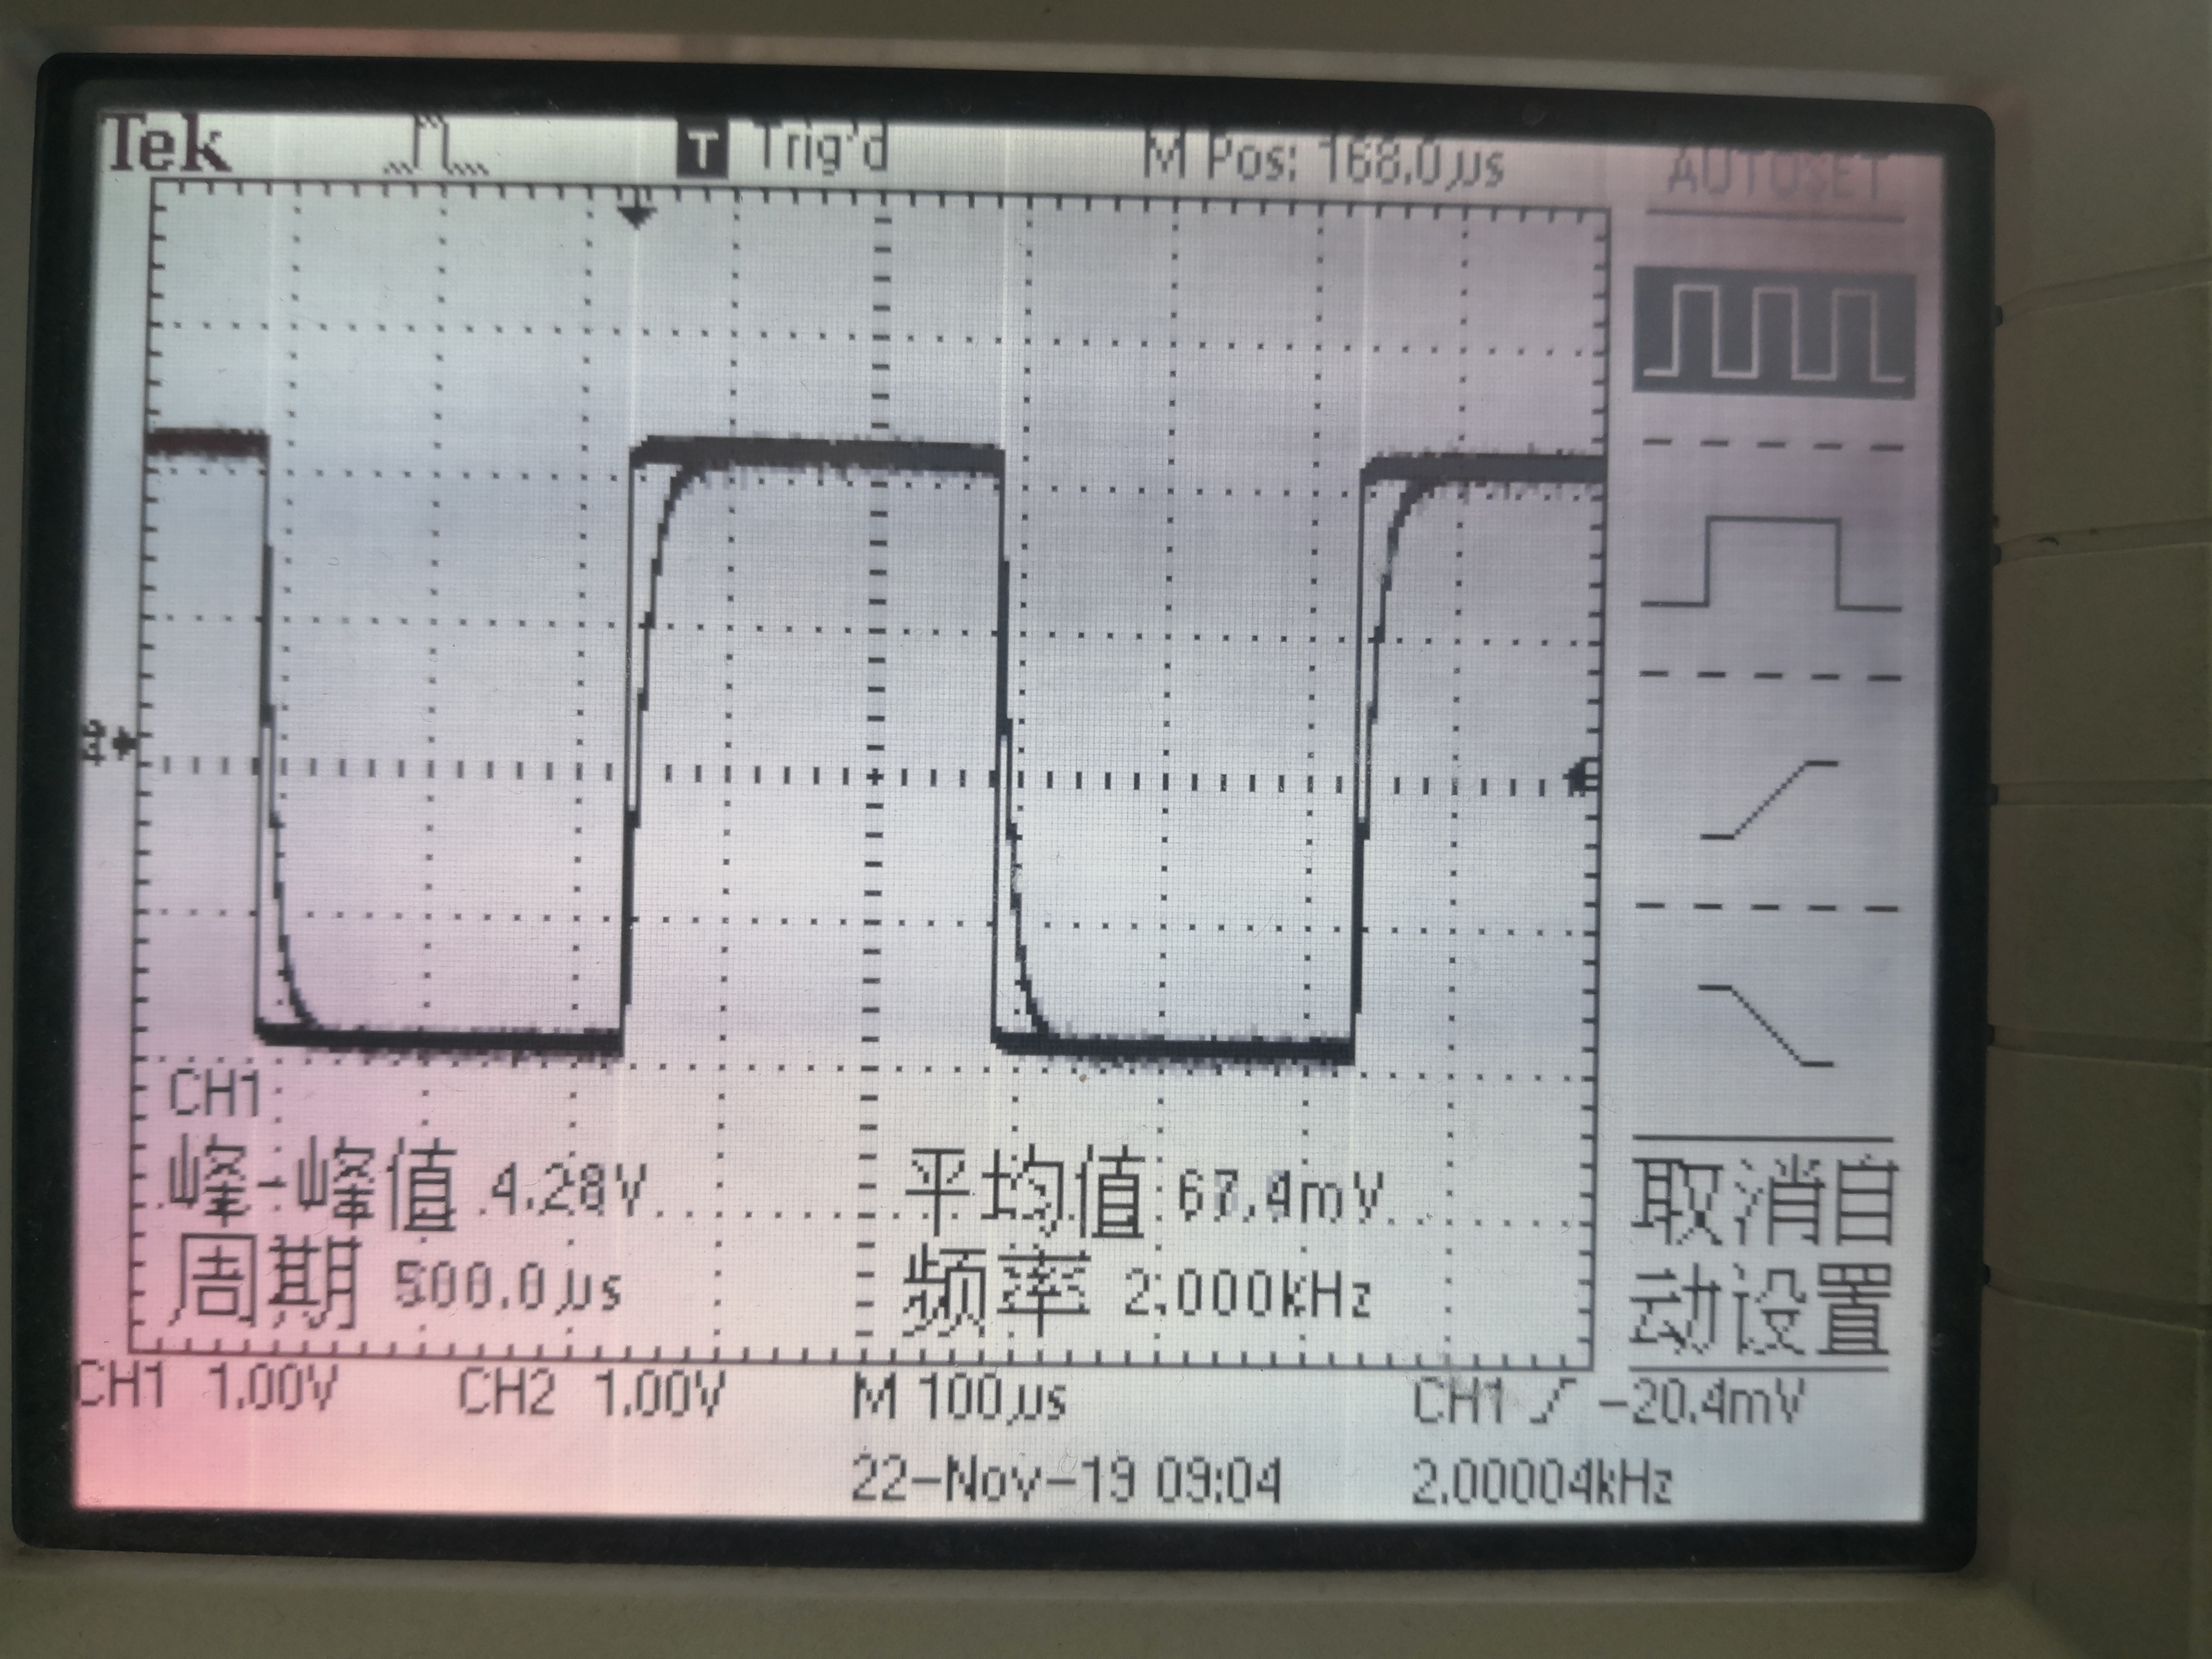
\includegraphics[scale=0.06]{1.jpg}
    \caption{Waveform of $U_C$ in $RC$ series circuit.}\label{FigRCC}
\end{figure}


The measured data for the $RC$ series are shown in Table \ref{TableRC}.

\begin{table}[H]
    \centering
    \begin{tabular}{lr|lr}
        \toprule
        $R\,\,[\Omega]$ & 100.63 $\pm$ 0.01 & $f\,\,[\text{Hz}]$                      & 2000.000 $\pm$ 0.001 \\
        $C$ [nF]        & 99.82 $\pm$ 0.01  & $\mathcal{E}\,\,[\text{V}_{\text{pp}}]$ & 4.000 $\pm$ 0.001    \\
                        &                   & $T_{1/2}\,\,[\mu\text{s}]$              & 9.000 $\pm$ 0.001    \\
        \bottomrule
    \end{tabular}
    \caption{$T_{1/2}$ measurement data for a $RC$ series circuit.\label{TableRC}}
\end{table}

According to Eq.\eqref{eq:ThalfRC}, the experimental time constant is then calculated as
$$\tau = \frac{T_{1/2}}{\ln 2} = \frac{9.000}{\ln 2} = 12.9842\pm 0.0014 \,\,[\mu\text{s}].$$

The theoretical time constant for the RC circuit is
$$\tau_{\text{theo}} = RC = 100.63 \times 99.82 \times 10^{-3} = 10.0449 \pm 0.0014 \,\,[\mu\text{s}].$$

The relative error is thus
$$\epsilon = \frac{\tau-\tau_{\text{theo}}}{\tau_{\text{theo}}} \times 100\% = \frac{12.9842 - 10.0449}{10.0449} \times 100\% = 29.26\%.$$

\subsection{$RL$ Series Circuit}

The waveform of the voltage across the resistance $U_R$ in the $RL$ circuit is recorded in Figure \ref{FigRLL}.
\begin{figure}[H]\centering
    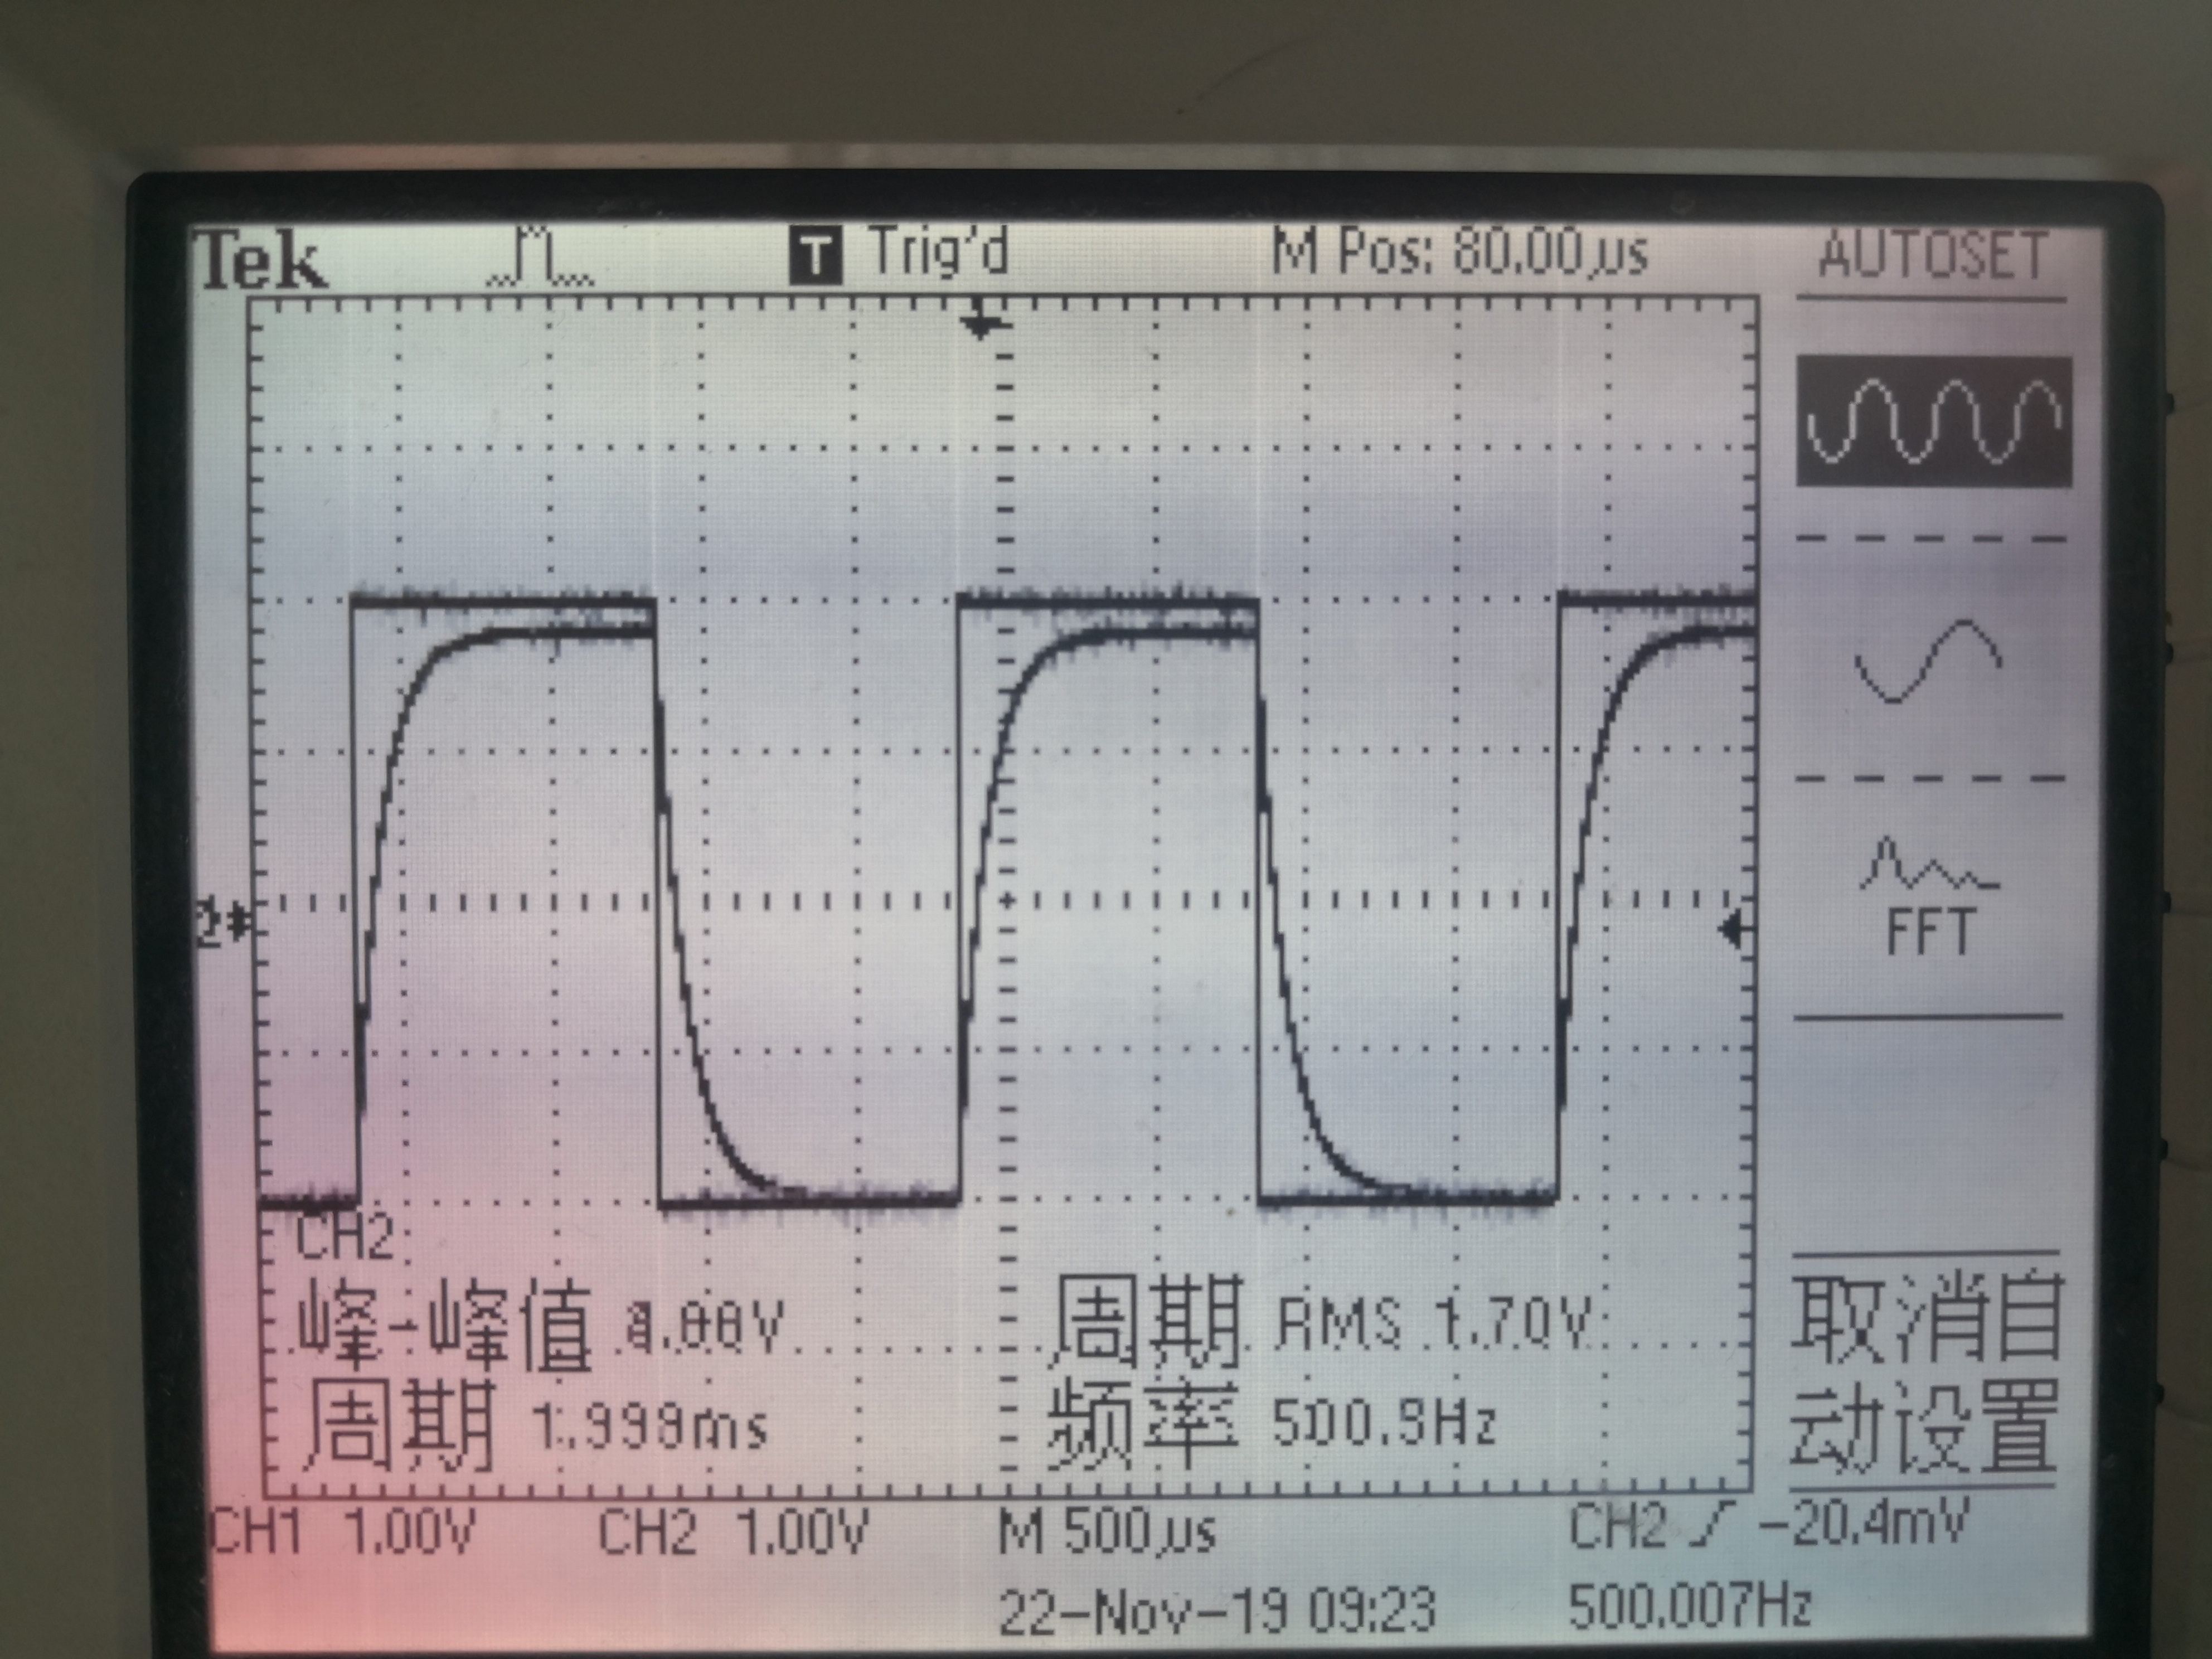
\includegraphics[scale=0.06]{2.jpg}
    \caption{Waveform of $U_R$ in $RL$ series circuit.}\label{FigRLL}
\end{figure}

The measured data for the $RL$ series are shown in Table \ref{TableRL}.

\begin{table}[H]
    \centering
    \begin{tabular}{lr|lr}
        \toprule
        $R\,\,[\Omega]$ & 100.63 $\pm$ 0.01 & $f\,\,[\text{Hz}]$                      & 500.000 $\pm$ 0.001 \\
        $L$ [H]         & 0.01 $\pm$ 0.00   & $\mathcal{E}\,\,[\text{V}_{\text{pp}}]$ & 4.000 $\pm$ 0.001   \\
                        &                   & $T_{1/2}\,\,[\mu\text{s}]$              & 72.00 $\pm$ 0.01    \\
        \bottomrule
    \end{tabular}
    \caption{$T_{1/2}$ measurement data for a $RL$ series circuit.\label{TableRL}}
\end{table}

According to the Eq.\eqref{eq:ThalfRL}, the experimental time constant is then calculated as
$$\tau = \frac{T_{1/2}}{\ln 2} = \frac{72.00}{\ln 2} = 103.874 \pm 0.014 \,\,[\mu\text{s}].$$

The theoretical time constant for the RL circuit is
$$\tau_{\text{theo}} = \frac{L}{R} = \frac{0.01}{100.63} \times 10^{6} = 99.374 \pm 0.010 \,\,[\mu\text{s}].$$

The relative error is thus
$$\epsilon = \frac{\tau-\tau_{\text{theo}}}{\tau_{\text{theo}}} \times 100\% = \frac{103.874 - 99.374}{99.374} \times 100\% = 4.53\%.$$

\subsection{$RLC$ Series Circuit}
The waveform of the voltage across the capacitor in the underdamped, critically damped and overdamped regimes of the $RLC$ series circuit.

\begin{figure}[H]\centering
    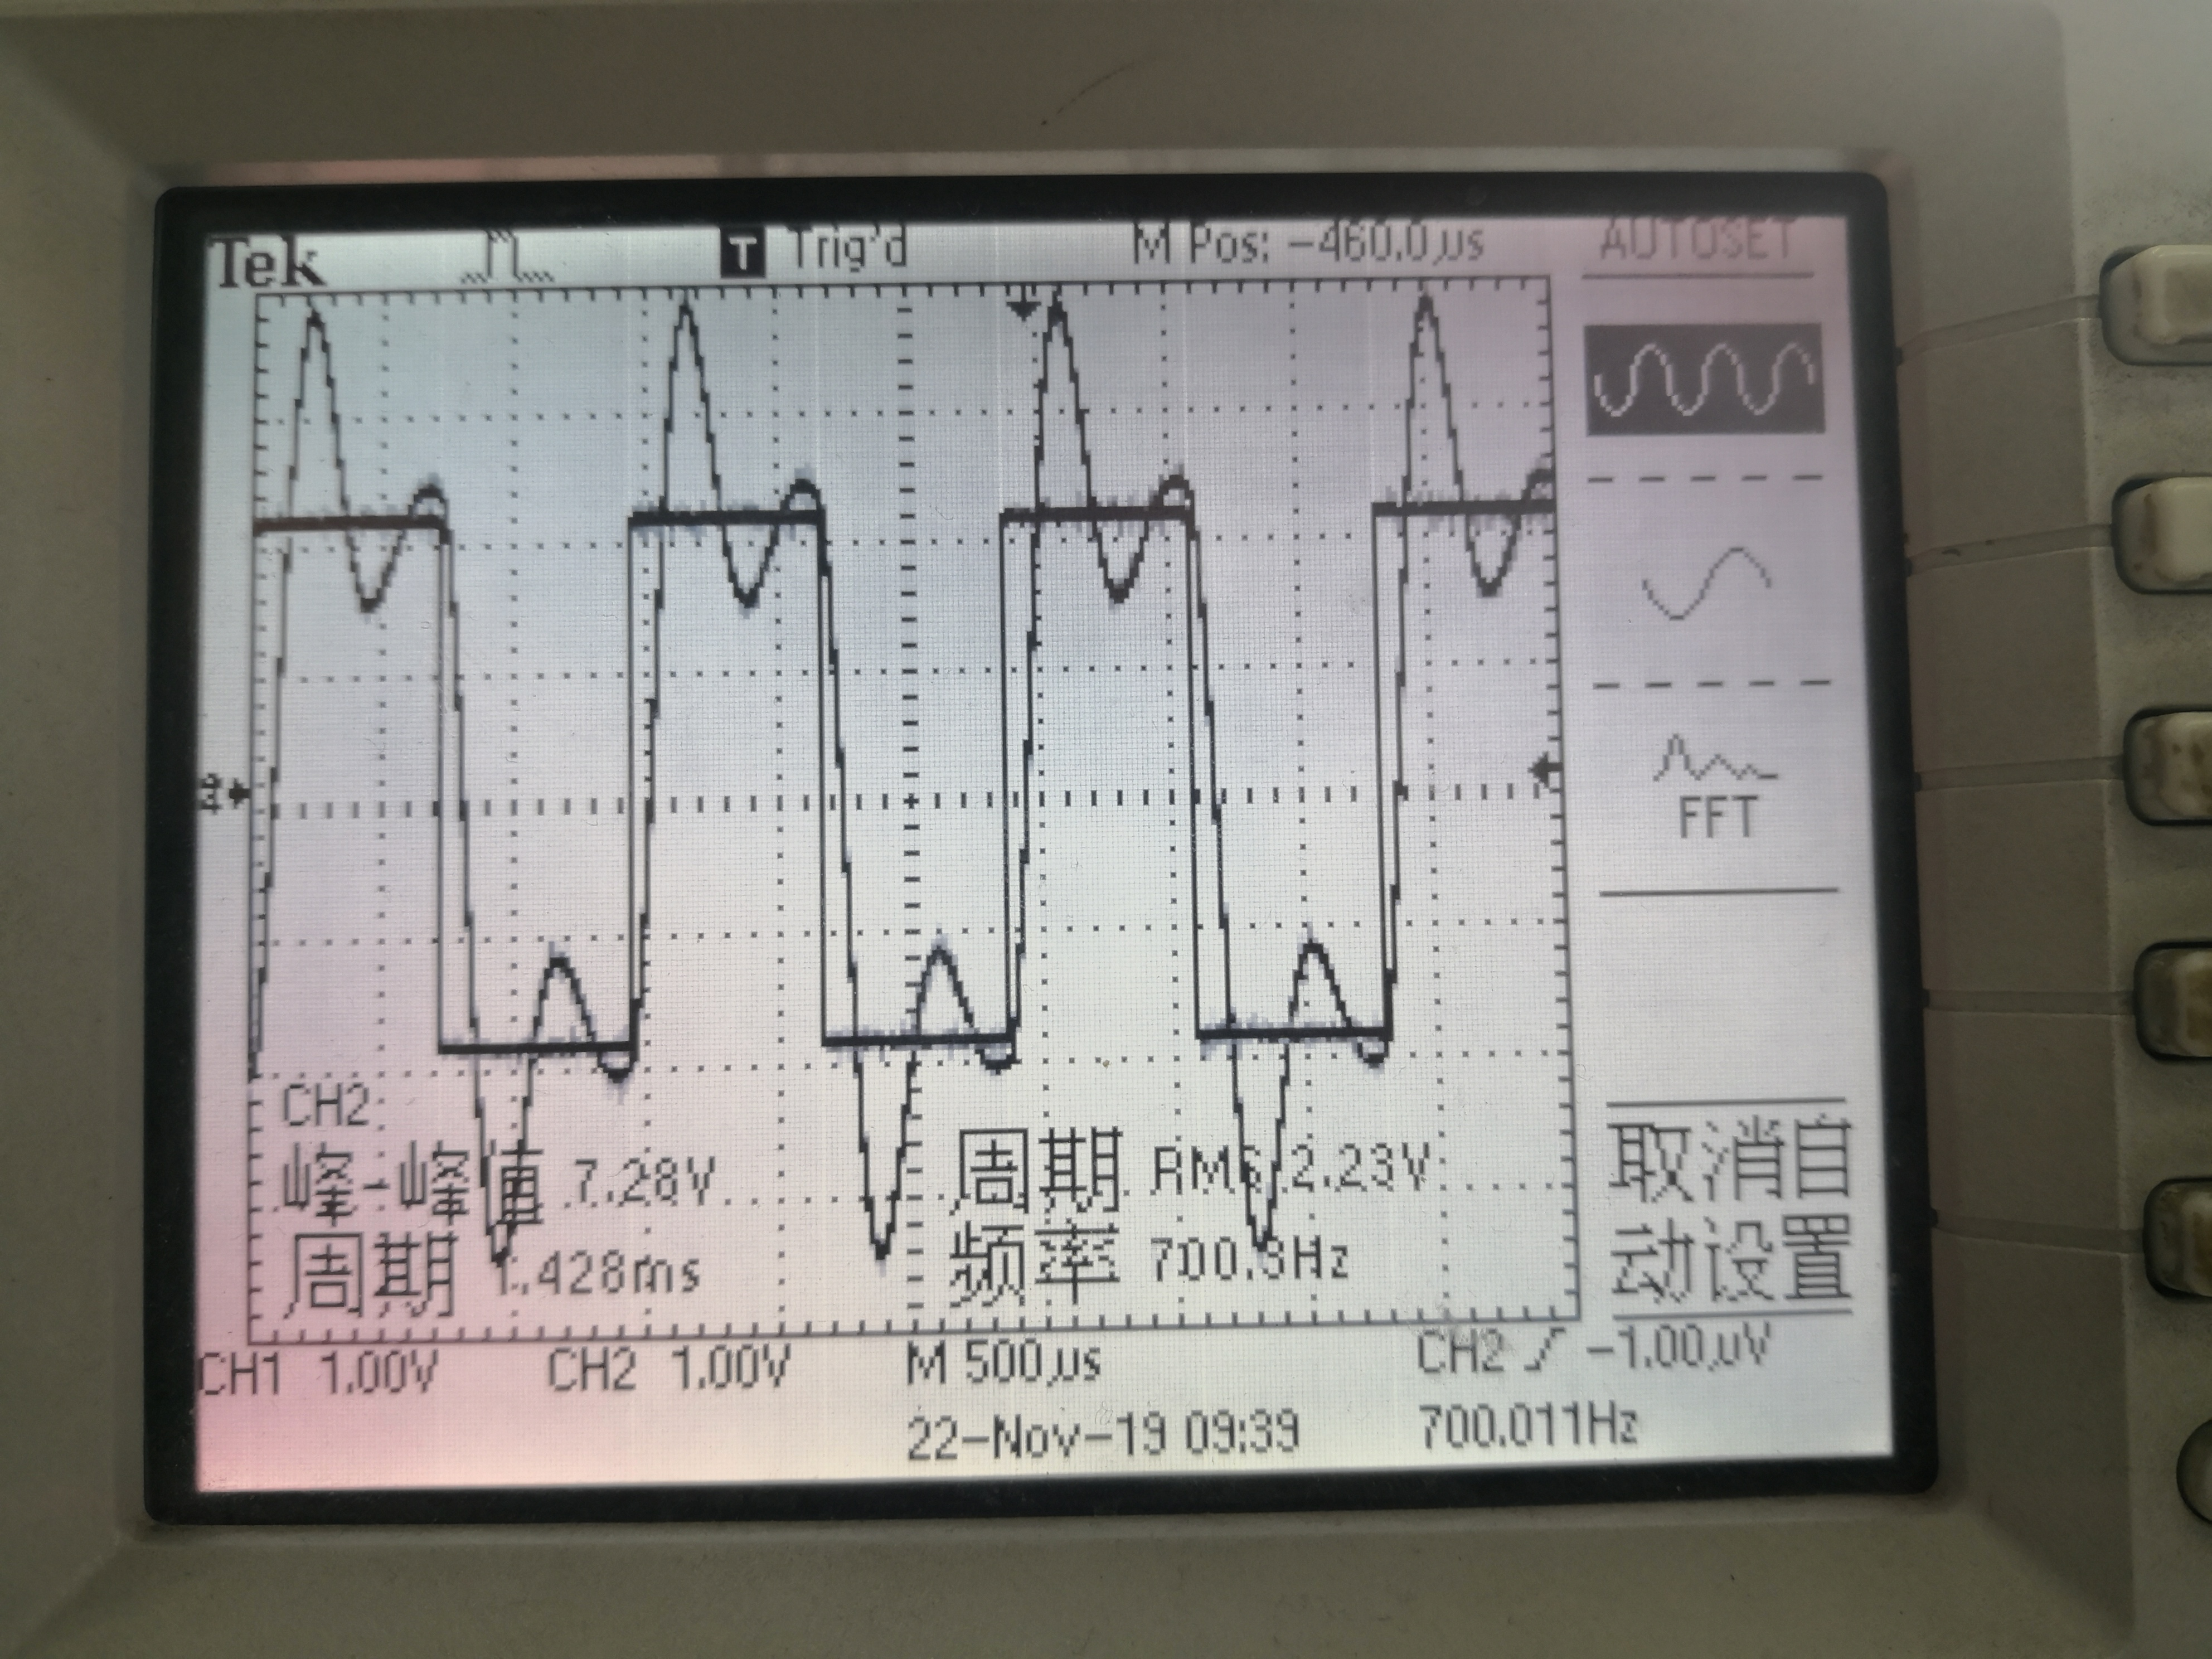
\includegraphics[scale=0.06]{3.jpg}
    \caption{Waveform of underdamped regime in a $RLC$ series circuit.}\label{FigUnderdamp}
\end{figure}

\begin{figure}[H]\centering
    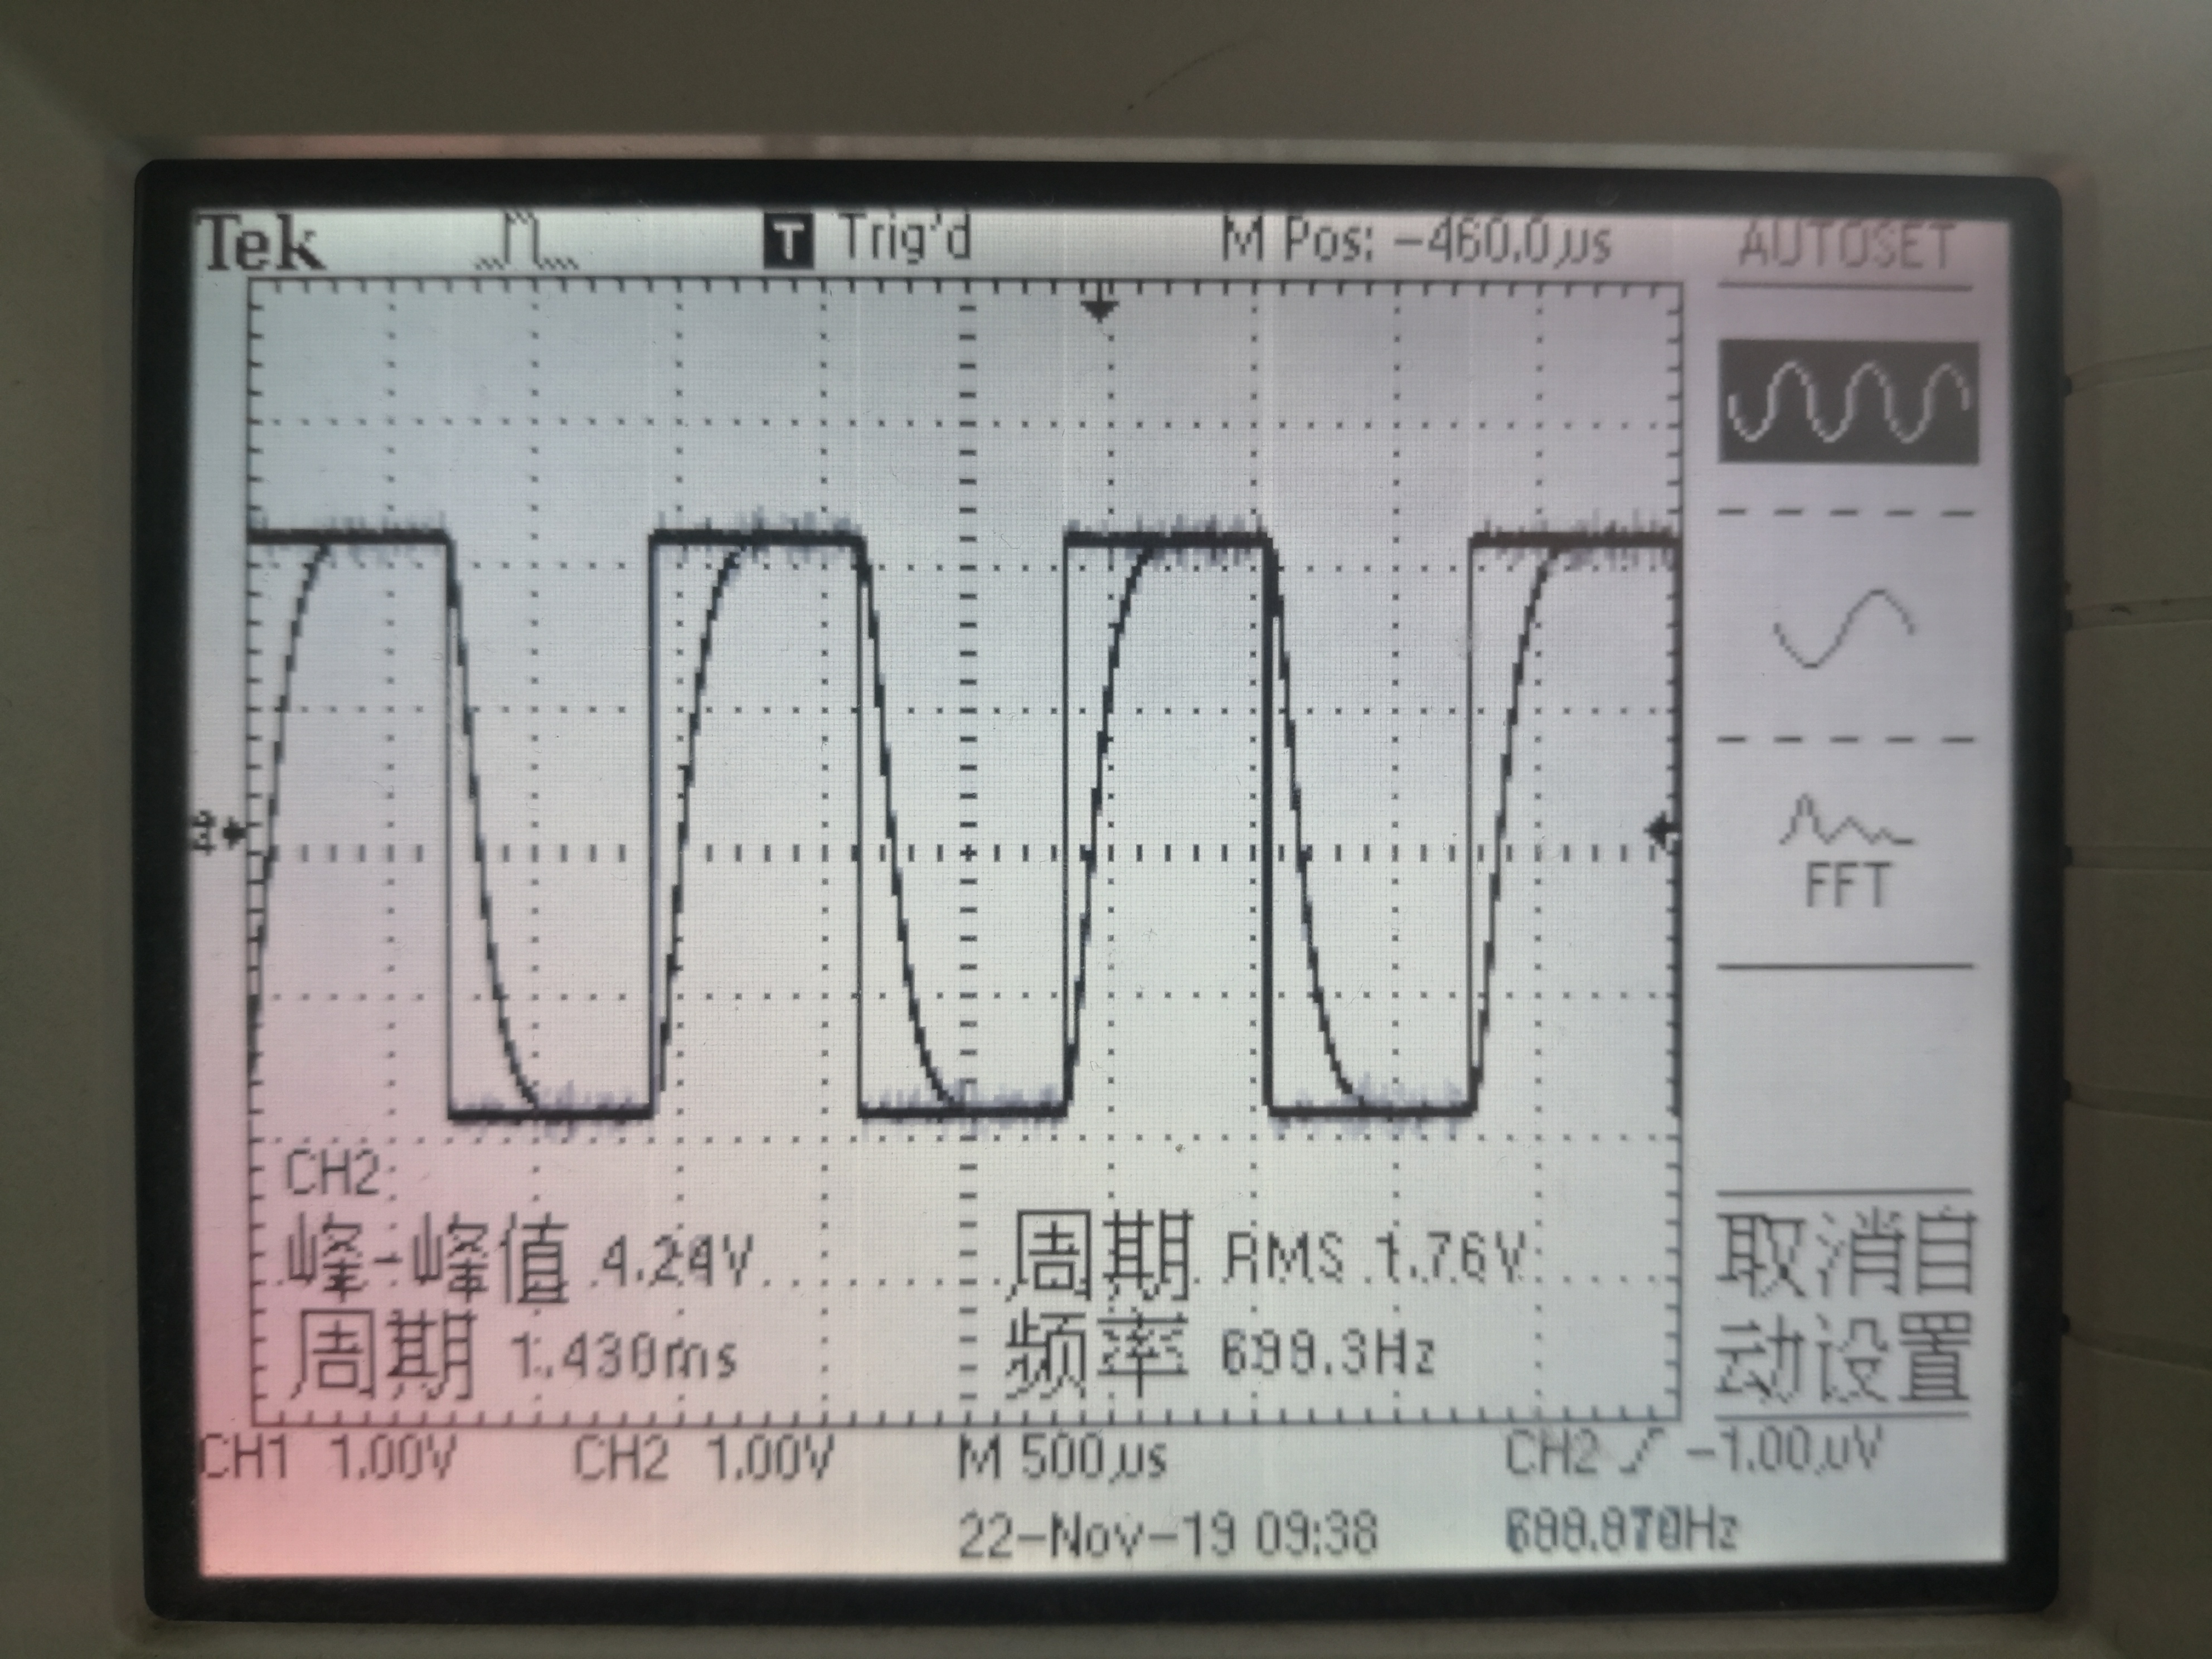
\includegraphics[scale=0.06]{4.jpg}
    \caption{Waveform of critically damped regime in a $RLC$ series circuit.}
\end{figure}

\begin{figure}[H]\centering
    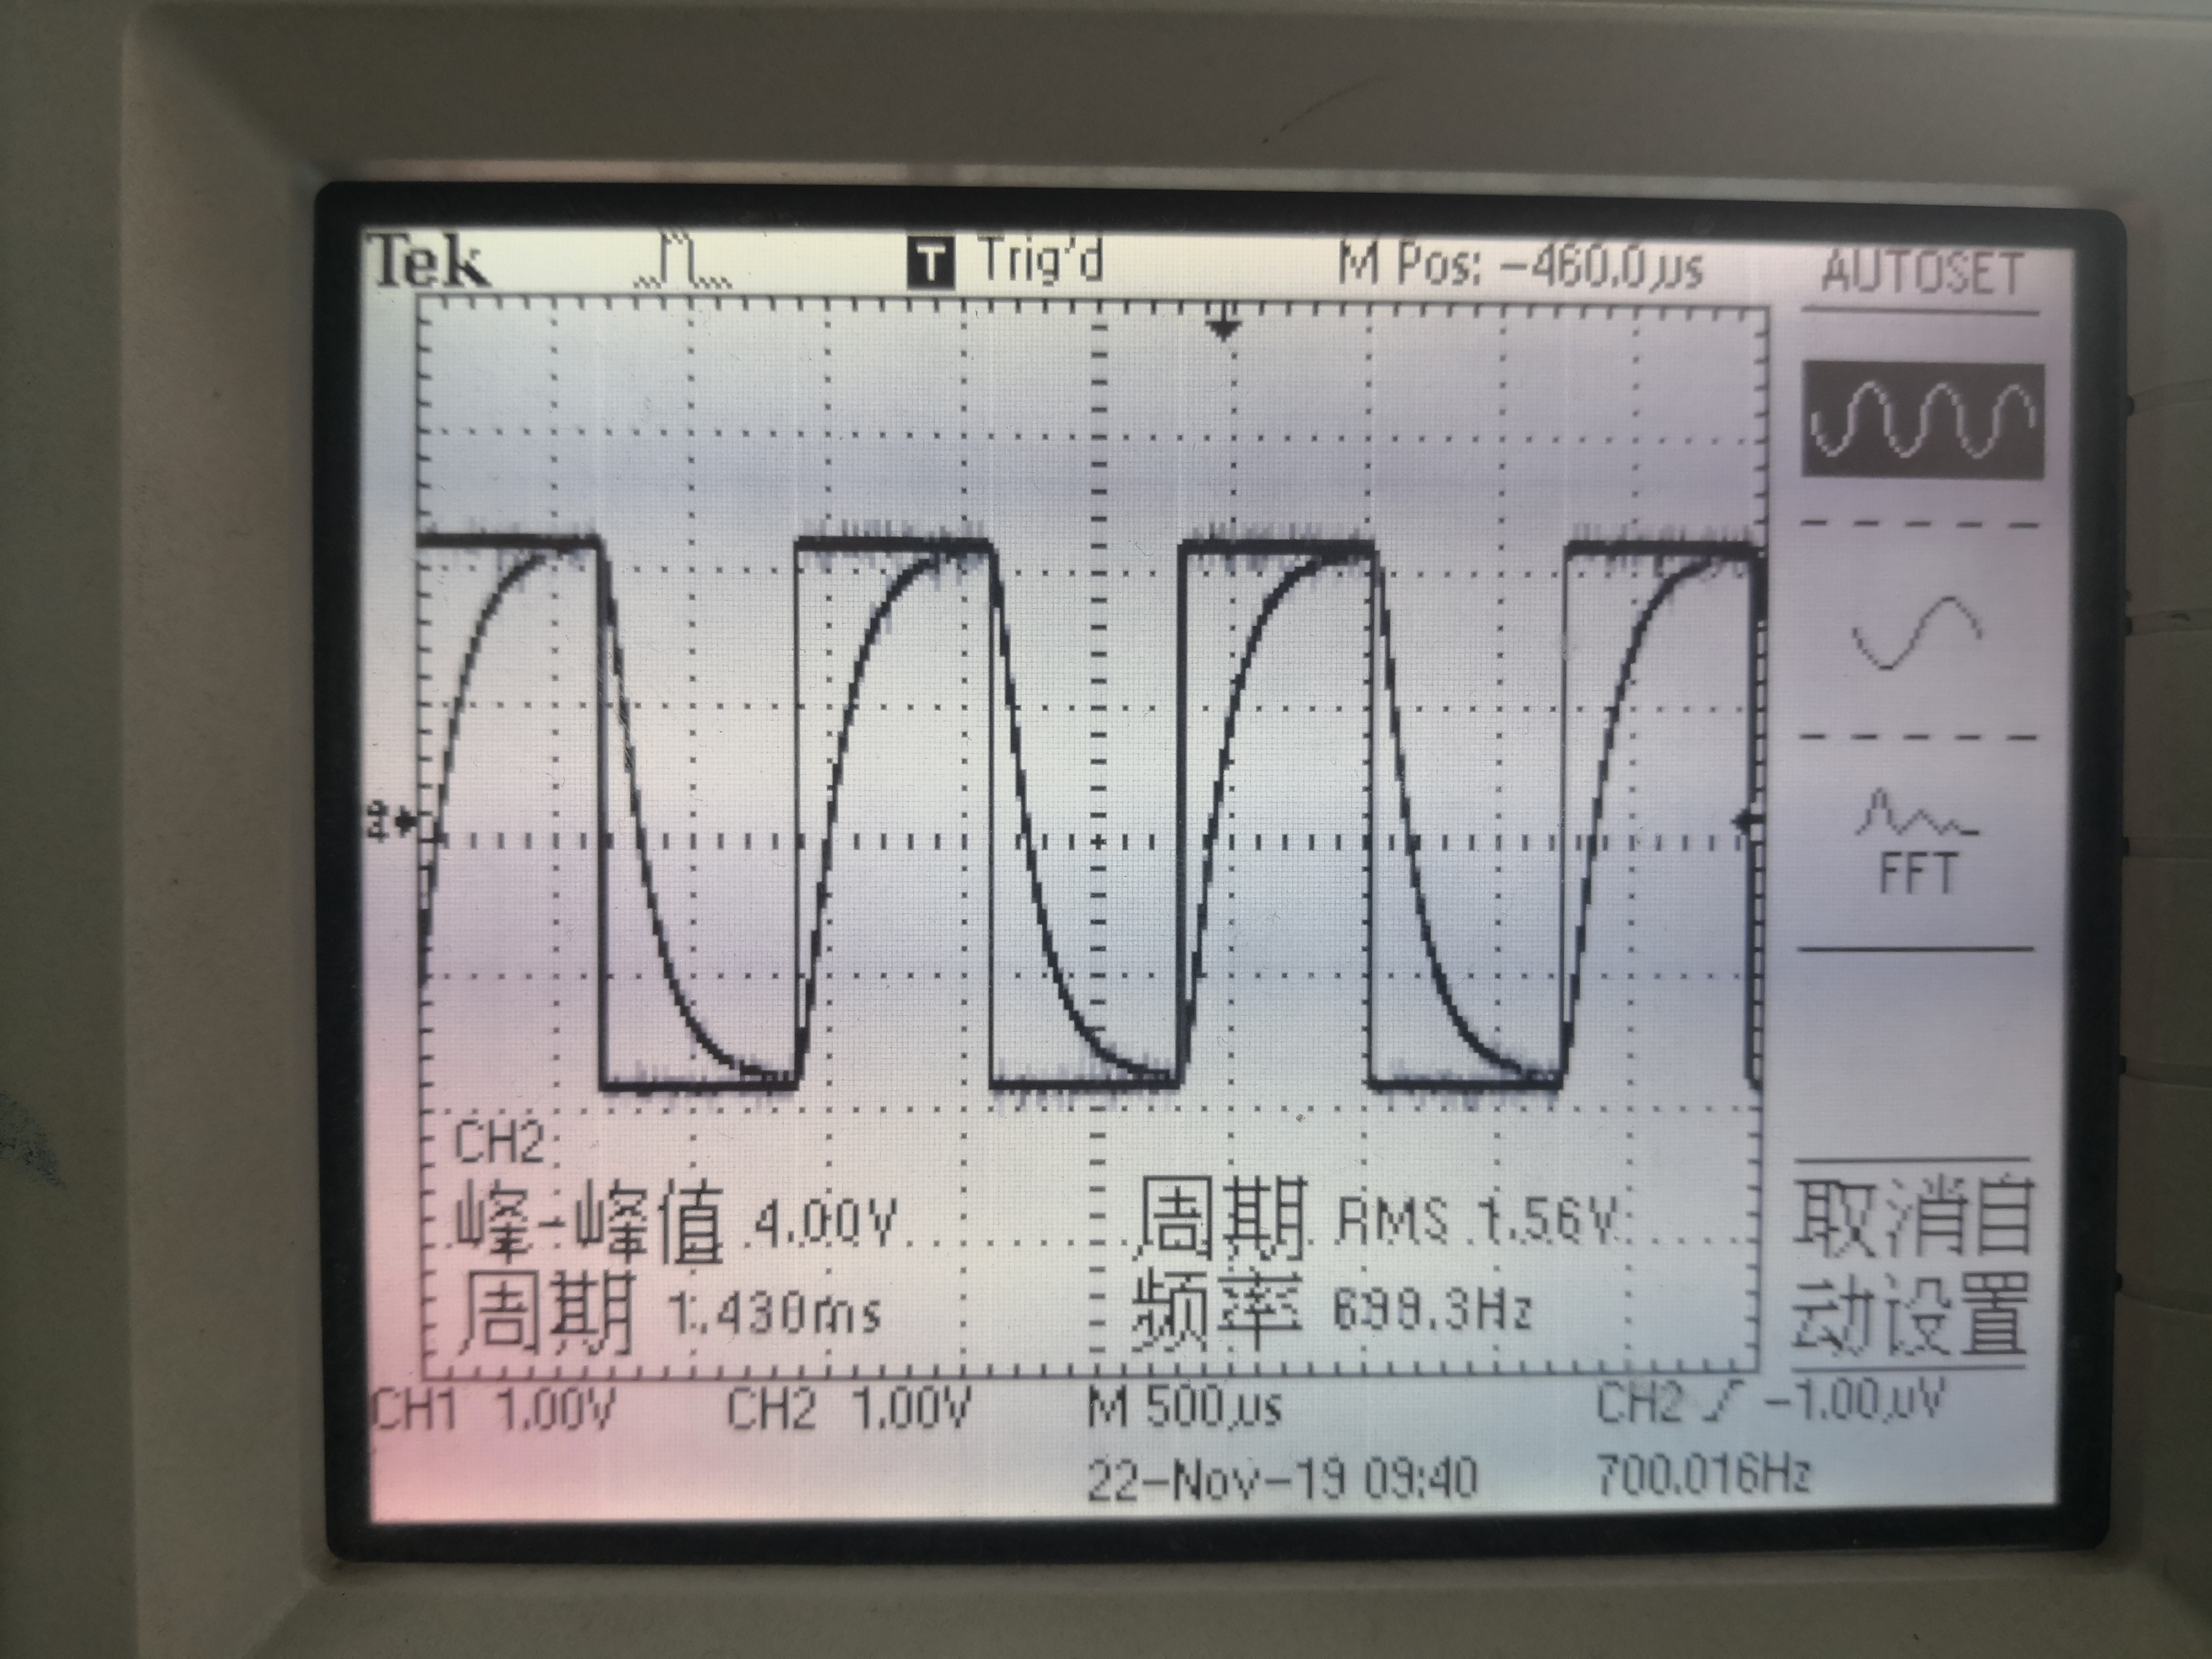
\includegraphics[scale=0.06]{5.jpg}
    \caption{Waveform of overdamped regime in a $RLC$ series circuit.}\label{FigOverdamp}
\end{figure}

The measured data for the $RLC$ circuit are shown in Table \ref{TableRLC}.

\begin{table}[H]\centering
    \begin{tabular}{lr|lr}
        \toprule
        $L$ [H]                               & 0.01 $\pm$ 0.00            & $\mathcal{E}\,\,[\text{V}_{\text{pp}}]$ & 4.000 $\pm$ 0.001   \\
        $C$ [nF]                              & 99.82 $\pm$ 0.01           & $f$ [Hz]                                & 700.000 $\pm$ 0.001 \\
        \multicolumn{2}{l|}{$\beta t = 1.68$} & $T_{1/2}\,\,[\mu\text{s}]$ & 120.0 $\pm$ 0.1                                               \\
        \bottomrule
    \end{tabular}
    \caption{$T_{1/2}$ measurement data for a critically damped $RLC$ series circuit.}\label{TableRLC}
\end{table}

Accordint to Eq.\eqref{eq:ThalfRLC}, the experimental time constant is then calculated as
$$\tau = T_{1/2}/1.68 = 120.0 \div 1.68 = 71.43 \pm 0.06\,\,[\mu\text{s}],$$

By the same equation, the theoretical time constant is
$$\tau_{\text{theo}} = \frac{1}{\beta} = \frac{1}{\omega_0} = \sqrt{LC} = \sqrt{0.01 \times 99.82 \times 10^{-9}} \times 10^{6} = 31.5943 \pm 0.0016 \,\,[\mu\text{s}].$$

The relative error is thus
$$\epsilon = \frac{\tau - \tau_{\text{theo}}}{\tau_{\text{theo}}} \times 100\% = \frac{71.43 - 31.5943}{31.5943} \times 100\% = 126.1\%.$$

\subsection{$RLC$ Resonant Circuit}

\subsubsection{Relation of $I/I_m$ vs. $f/f_0$ and $\varphi$ vs. $f/f_0$}

The measured data for the $RLC$ resonant circuit are shown in Table \ref{TableResonant}.
\begin{table}[H]\centering
    \begin{tabular}{ccc}
        \toprule
        \multicolumn{2}{l}{$R\,\,[\Omega]$ 100.63 $\pm$ 0.01} &                                                                                                           \\
        \multicolumn{2}{l}{$L$ [H] 0.01 $\pm$ 0.00}           & \multicolumn{1}{l}{$\mathcal{E}\,\,[\text{V}_{\text{pp}}]$ 4.000 $\pm$ 0.001}                             \\
        \multicolumn{2}{l}{$C$ [nF] 99.82 $\pm$ 0.01}         & \multicolumn{1}{l}{$f_0$ [Hz] 5000.000 $\pm$ 0.001}                                                       \\
        \midrule
                                                              & $U_R\,\,[\text{V}_\text{pp}] \pm 0.02/0.002\,\,[\text{V}_\text{pp}]$          & $f$ [Hz] $\pm$ 0.001 [Hz] \\
        \midrule
        1                                                     & 0.920 $\pm 0.002$                                                             & 2500.000                  \\
        2                                                     & 1.24  $\pm 0.02$                                                              & 3000.000                  \\
        3                                                     & 1.64  $\pm 0.02$                                                              & 3500.000                  \\
        4                                                     & 2.04  $\pm 0.02$                                                              & 3800.000                  \\
        5                                                     & 2.48  $\pm 0.02$                                                              & 4100.000                  \\
        6                                                     & 2.86  $\pm 0.02$                                                              & 4300.000                  \\
        7                                                     & 3.22  $\pm 0.02$                                                              & 4500.000                  \\
        8                                                     & 3.58  $\pm 0.02$                                                              & 4700.000                  \\
        9                                                     & 3.70  $\pm 0.02$                                                              & 4800.000                  \\
        10                                                    & 3.76  $\pm 0.02$                                                              & 4900.000                  \\
        11                                                    & 3.80  $\pm 0.02$                                                              & 5000.000                  \\
        12                                                    & 3.78  $\pm 0.02$                                                              & 5100.000                  \\
        13                                                    & 3.74  $\pm 0.02$                                                              & 5200.000                  \\
        14                                                    & 3.66  $\pm 0.02$                                                              & 5300.000                  \\
        15                                                    & 3.38  $\pm 0.02$                                                              & 5500.000                  \\
        16                                                    & 3.12  $\pm 0.02$                                                              & 5700.000                  \\
        17                                                    & 2.80  $\pm 0.02$                                                              & 5900.000                  \\
        18                                                    & 2.42  $\pm 0.02$                                                              & 6200.000                  \\
        19                                                    & 2.14  $\pm 0.02$                                                              & 6500.000                  \\
        20                                                    & 1.78  $\pm 0.02$                                                              & 7000.000                  \\
        21                                                    & 1.50  $\pm 0.02$                                                              & 7500.000                  \\
        \bottomrule
    \end{tabular}
    \caption{Measurement data for the $U_R$ vs. $f$ dependence for a $RLC$ resonant circuit.}\label{TableResonant}
\end{table}

As illustrated in the procedure part, to study the feature of resonance, we intend to plot $I/I_m$ vs. $f/f_0$ and $\varphi$ vs. $f/f_0$. To achieve that, first obtain from Table \ref{TableResonant} that $U_R$ reaches its maximum $U_m = 3.80\,V_{\text{pp}}$ when the frequency is 5000.000 Hz. This implies that the experimental estimated resonance frequency $f_0 = 5000.000\pm 0.001\,Hz$.

Then the values of $f/f_0$ and $I/I_m$ are calculted. Take the first set of data as an example,
$$f/f_0 = \frac{2500.000}{5000.000} = 0.500 \pm 0.0000002.$$
$$I/I_\text{m} = U_R/U_\text{m} = \frac{0.920}{3.80} = 0.2421 \pm 0.0014.$$
All the results for other calculations are shown in Table \ref{TablePhi}.

For the phase difference $\varphi$, as discussed in the introduction part, there are two ways to obtain its value.

On the one hand, through Eq.\eqref{eq:phitheo}, the ``theoretical'' value of phase difference is obtained. Take the first set of data as an example,
\begin{align*}
    \varphi_{theo} & = \tan^{-1}\bigg(\frac{2\pi fL - \frac{1}{2\pi fC}}{R}\bigg)                                                                 \\
                   & = \tan^{-1}\bigg(\frac{2\pi\times 2500.000\times 0.01-\frac{1}{2\pi \times 2500.000\times 99.82\times10^{-9}}}{100.63}\bigg) \\
                   & =  -1.36227 \pm 0.00003 \,[\text{rad}],
\end{align*}
All the results for other calculations are shown in Table \ref{TablePhi}.\\

On the other hand, the ``experimental'' value of phase difference can be deduced from Eq.\eqref{eq:phiex}. Take the first set of data as an example,
$$\varphi_\text{ex} = \cos^{-1}\frac{U_R}{U_m} = \cos^{-1}\frac{0.920}{3.80} = 1.3263 \pm 0.0014 \,[\text{rad}],$$
All the results for other calculations are shown in Table \ref{TablePhi}.

\begin{table}[H]\centering
    \begin{tabular}{ccccc}
        \toprule
           & $f/f_0$               & $I/I_\text{m}$      & $\varphi_\text{theo}\,[\text{rad}]$ & $\varphi_\text{ex}\,[\text{rad}]$ \\
        \midrule
        1  & 0.500 $\pm$ 0.0000002 & 0.2421 $\pm$ 0.0014 & -1.36227 $\pm$ 0.00003              & 1.3263 $\pm$ 0.0014               \\
        2  & 0.600 $\pm$ 0.0000002 & 0.326  $\pm$ 0.006  & -1.28200 $\pm$ 0.00005              & 1.238  $\pm$ 0.006                \\
        3  & 0.700 $\pm$ 0.0000002 & 0.432  $\pm$ 0.006  & -1.16149 $\pm$ 0.00008              & 1.125  $\pm$ 0.006                \\
        4  & 0.760 $\pm$ 0.0000003 & 0.537  $\pm$ 0.006  & -1.05492 $\pm$ 0.00011              & 1.004  $\pm$ 0.007                \\
        5  & 0.820 $\pm$ 0.0000003 & 0.653  $\pm$ 0.006  & -0.90508 $\pm$ 0.00015              & 0.860  $\pm$ 0.008                \\
        6  & 0.860 $\pm$ 0.0000003 & 0.753  $\pm$ 0.007  & -0.77029 $\pm$ 0.00019              & 0.719  $\pm$ 0.010                \\
        7  & 0.900 $\pm$ 0.0000003 & 0.847  $\pm$ 0.007  & -0.5992  $\pm$ 0.0002               & 0.560  $\pm$ 0.013                \\
        8  & 0.940 $\pm$ 0.0000003 & 0.942  $\pm$ 0.007  & -0.3886  $\pm$ 0.0003               & 0.34   $\pm$ 0.02                 \\
        9  & 0.960 $\pm$ 0.0000003 & 0.974  $\pm$ 0.007  & -0.2705  $\pm$ 0.0003               & 0.23   $\pm$ 0.03                 \\
        10 & 0.980 $\pm$ 0.0000003 & 0.989  $\pm$ 0.007  & -0.1470  $\pm$ 0.0003               & 0.15   $\pm$ 0.05                 \\
        11 & 1.000 $\pm$ 0.0000003 & 1.000  $\pm$ 0.007  & -0.0214  $\pm$ 0.0003               & 0.00   $\pm$ /                    \\
        12 & 1.020 $\pm$ 0.0000003 & 0.995  $\pm$ 0.007  & 0.1023   $\pm$ 0.0003               & 0.10   $\pm$ 0.07                 \\
        13 & 1.040 $\pm$ 0.0000003 & 0.984  $\pm$ 0.007  & 0.2207   $\pm$ 0.0003               & 0.18   $\pm$ 0.04                 \\
        14 & 1.060 $\pm$ 0.0000003 & 0.963  $\pm$ 0.007  & 0.3311   $\pm$ 0.0003               & 0.27   $\pm$ 0.03                 \\
        15 & 1.100 $\pm$ 0.0000003 & 0.889  $\pm$ 0.007  & 0.5230   $\pm$ 0.0002               & 0.475  $\pm$ 0.015                \\
        16 & 1.140 $\pm$ 0.0000003 & 0.821  $\pm$ 0.007  & 0.67575  $\pm$ 0.00018              & 0.608  $\pm$ 0.012                \\
        17 & 1.180 $\pm$ 0.0000003 & 0.737  $\pm$ 0.007  & 0.79530  $\pm$ 0.00014              & 0.742  $\pm$ 0.010                \\
        18 & 1.240 $\pm$ 0.0000003 & 0.637  $\pm$ 0.006  & 0.92833  $\pm$ 0.00011              & 0.880  $\pm$ 0.008                \\
        19 & 1.300 $\pm$ 0.0000003 & 0.563  $\pm$ 0.006  & 1.02338  $\pm$ 0.00008              & 0.973  $\pm$ 0.007                \\
        20 & 1.400 $\pm$ 0.0000003 & 0.468  $\pm$ 0.006  & 1.13103  $\pm$ 0.00006              & 1.083  $\pm$ 0.007                \\
        21 & 1.500 $\pm$ 0.0000004 & 0.395  $\pm$ 0.006  & 1.20198  $\pm$ 0.00004              & 1.165  $\pm$ 0.006                \\
        \bottomrule
    \end{tabular}
    \caption{Results for $\varphi$, $f/f_0$ and $I/I_\text{m}$.}\label{TablePhi}
\end{table}

Then the $I/I_\text{m}$ vs. $f/f_0$, $\varphi_{\text{theo}}$ vs. $f/f_0$ and $\varphi_\text{ex}$ vs. $f/f_0$ relation are then plotted and presented in Figure \ref{FigIIm}$\sim$\ref{FigPhi_ex} respectively. Note that the values of $\varphi_\text{ex}$ are taken to be the negative of the original value when $f/f_0 < 1$ so that the plotted figure assumes similar shape as that for $\varphi_{\text{theo}}$.

\begin{figure}[H]\centering
    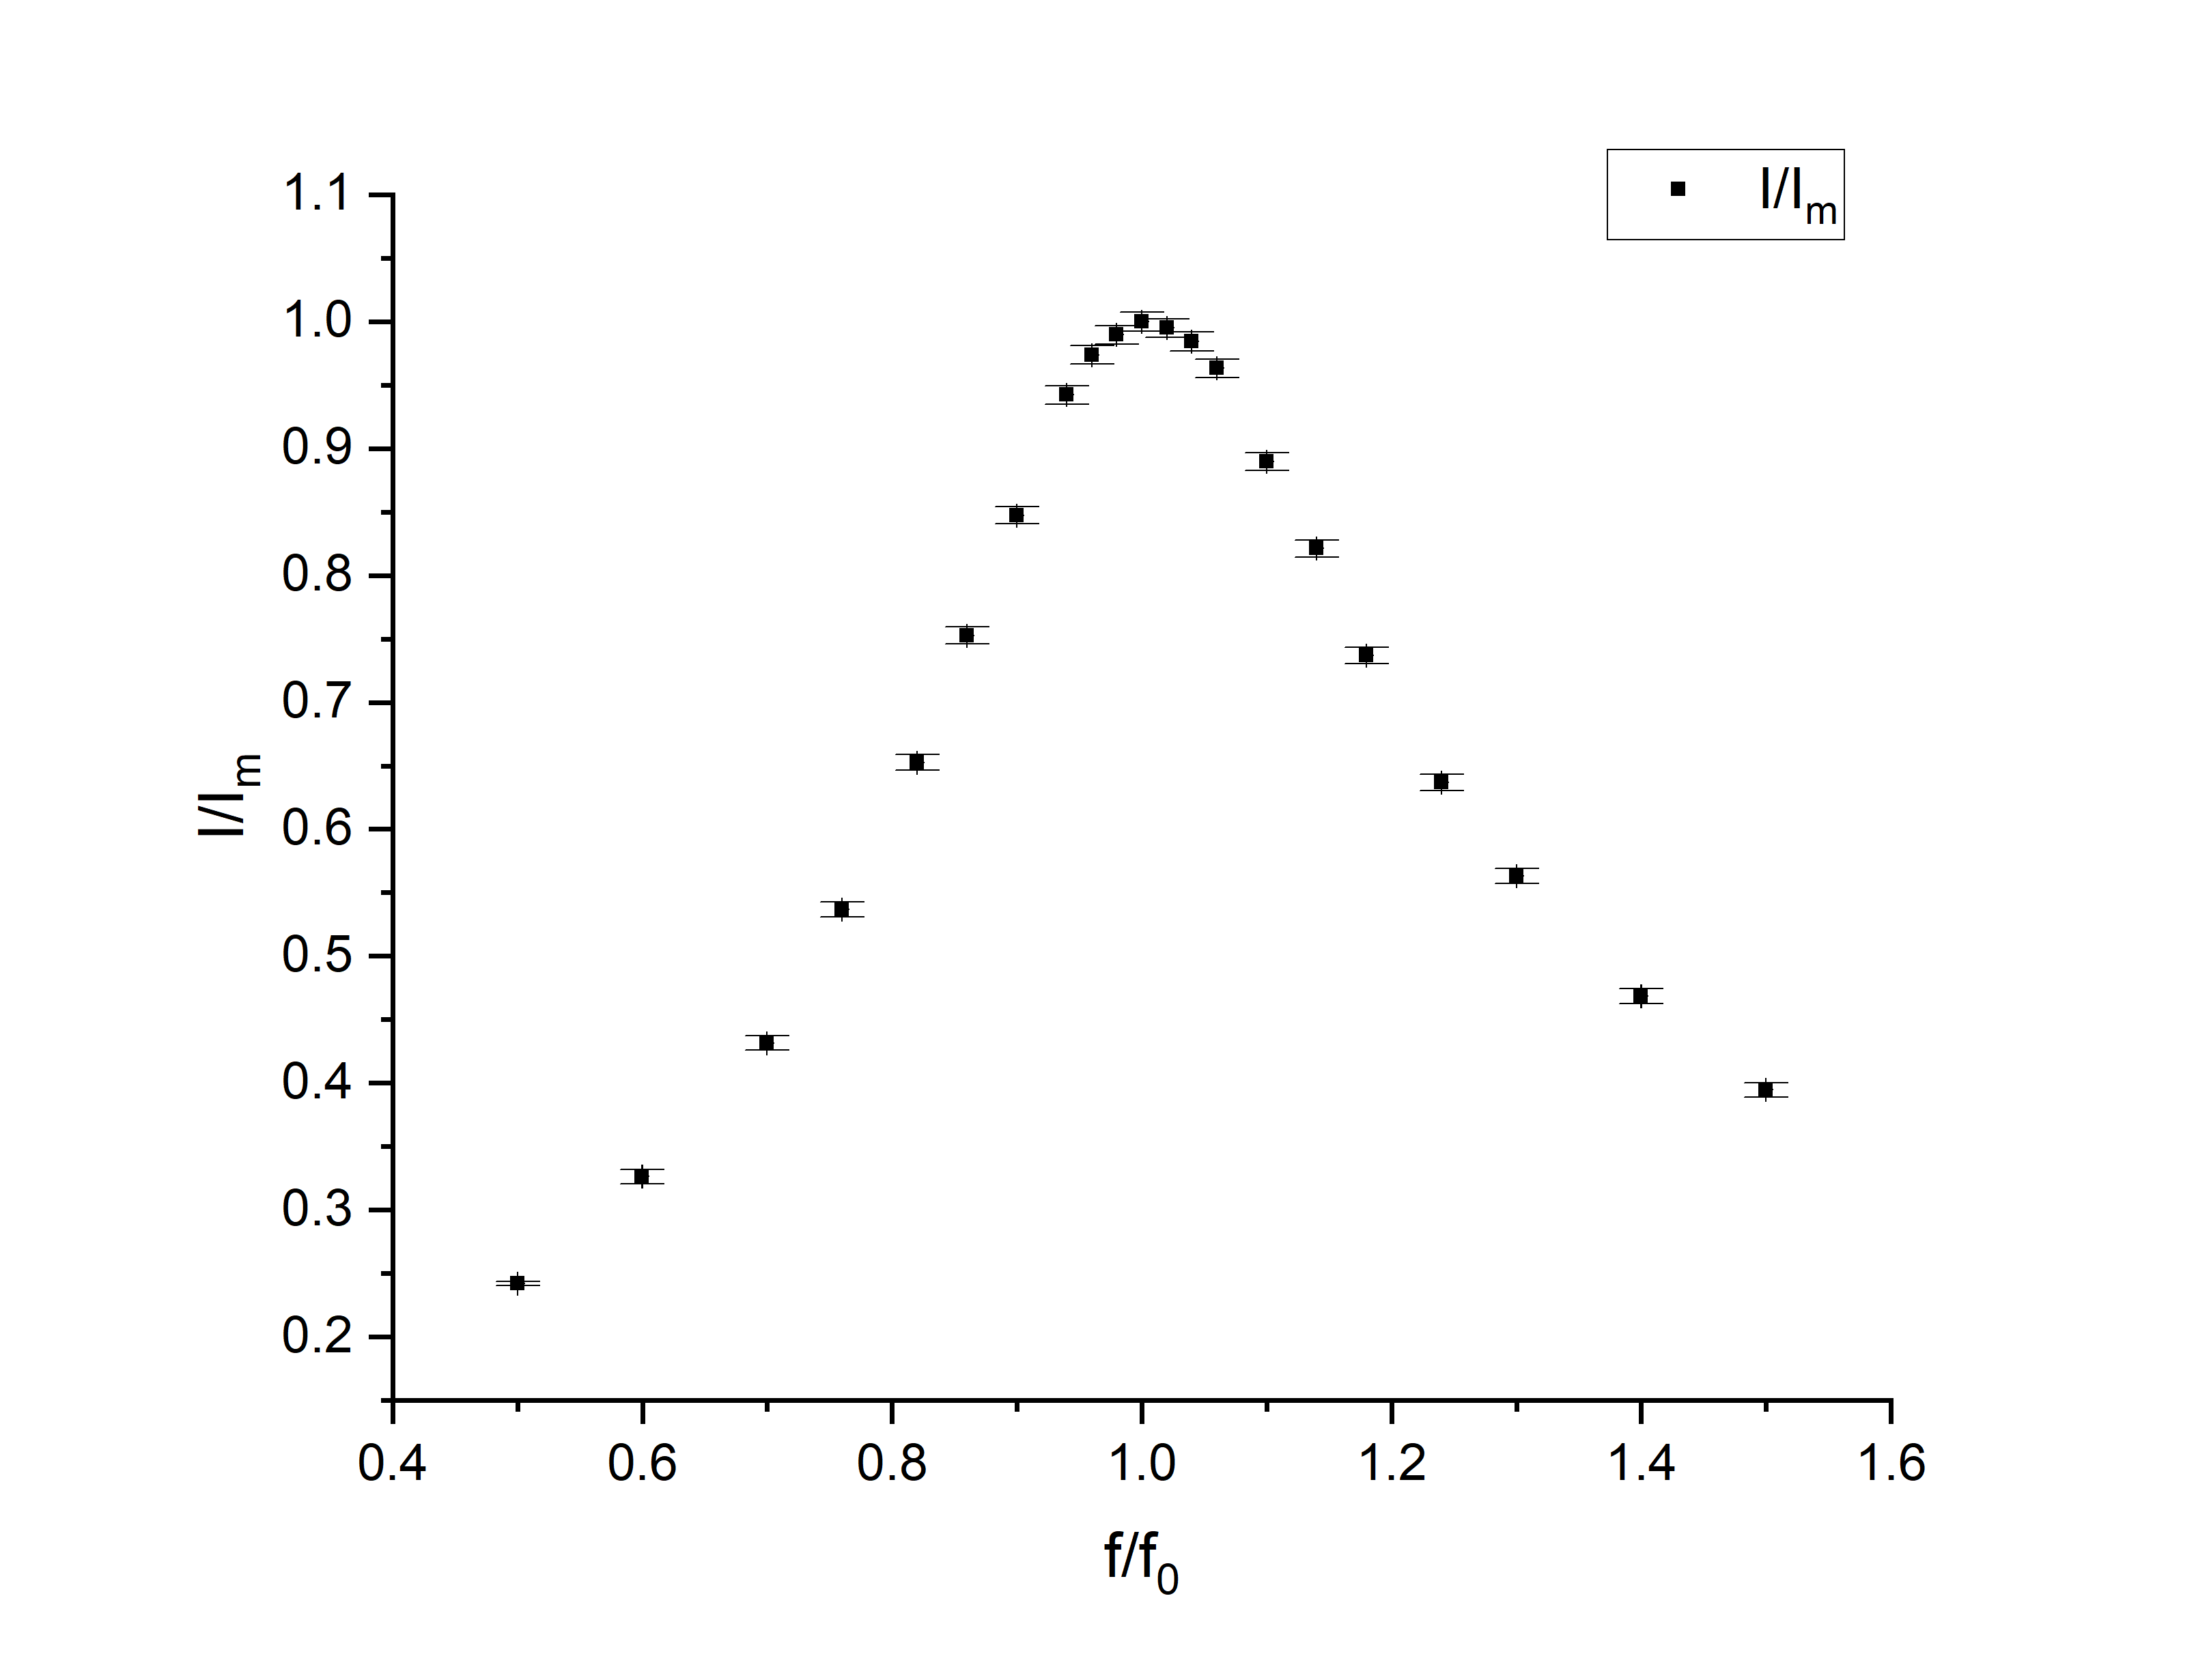
\includegraphics[scale=0.38]{IImff0.png}
    \caption{$I/I_\text{m}$ vs. $f/f_0$ relation.}\label{FigIIm}
\end{figure}

\begin{figure}[H]\centering
    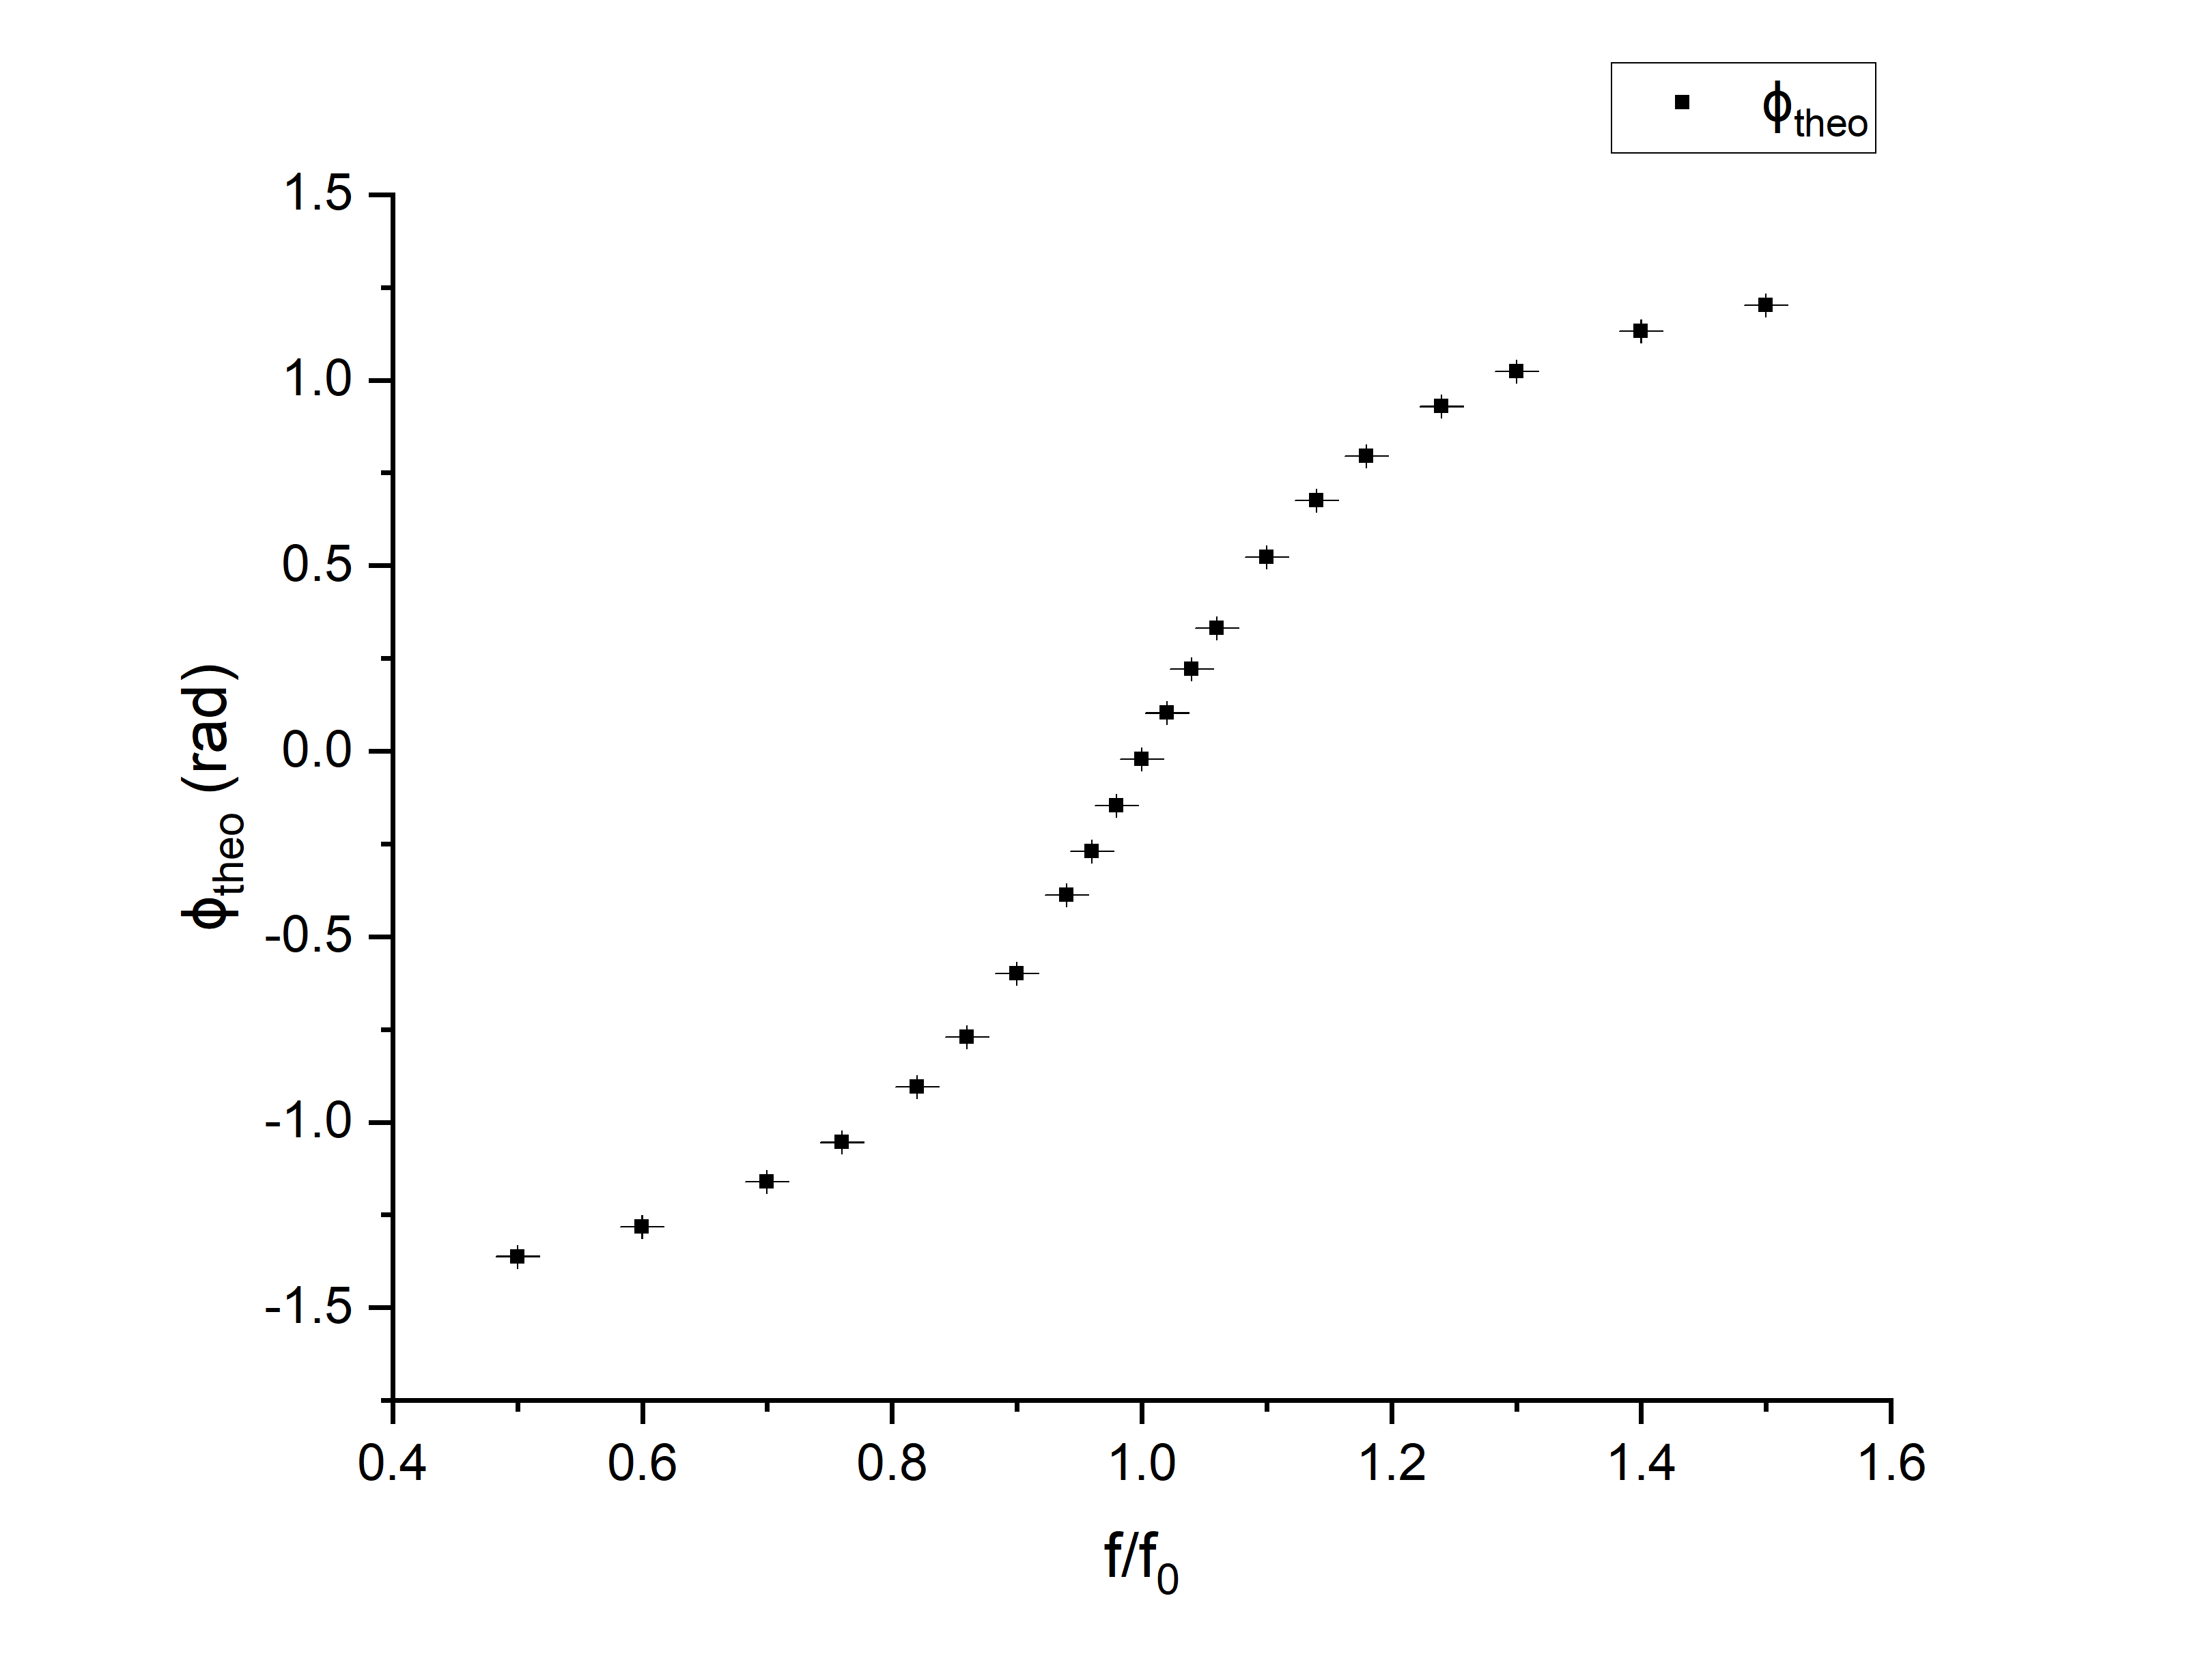
\includegraphics[scale=0.37]{phi.png}
    \caption{$\varphi$ vs. $f/f_0$ relation.}\label{FigPhi}
\end{figure}

\begin{figure}[H]\centering
    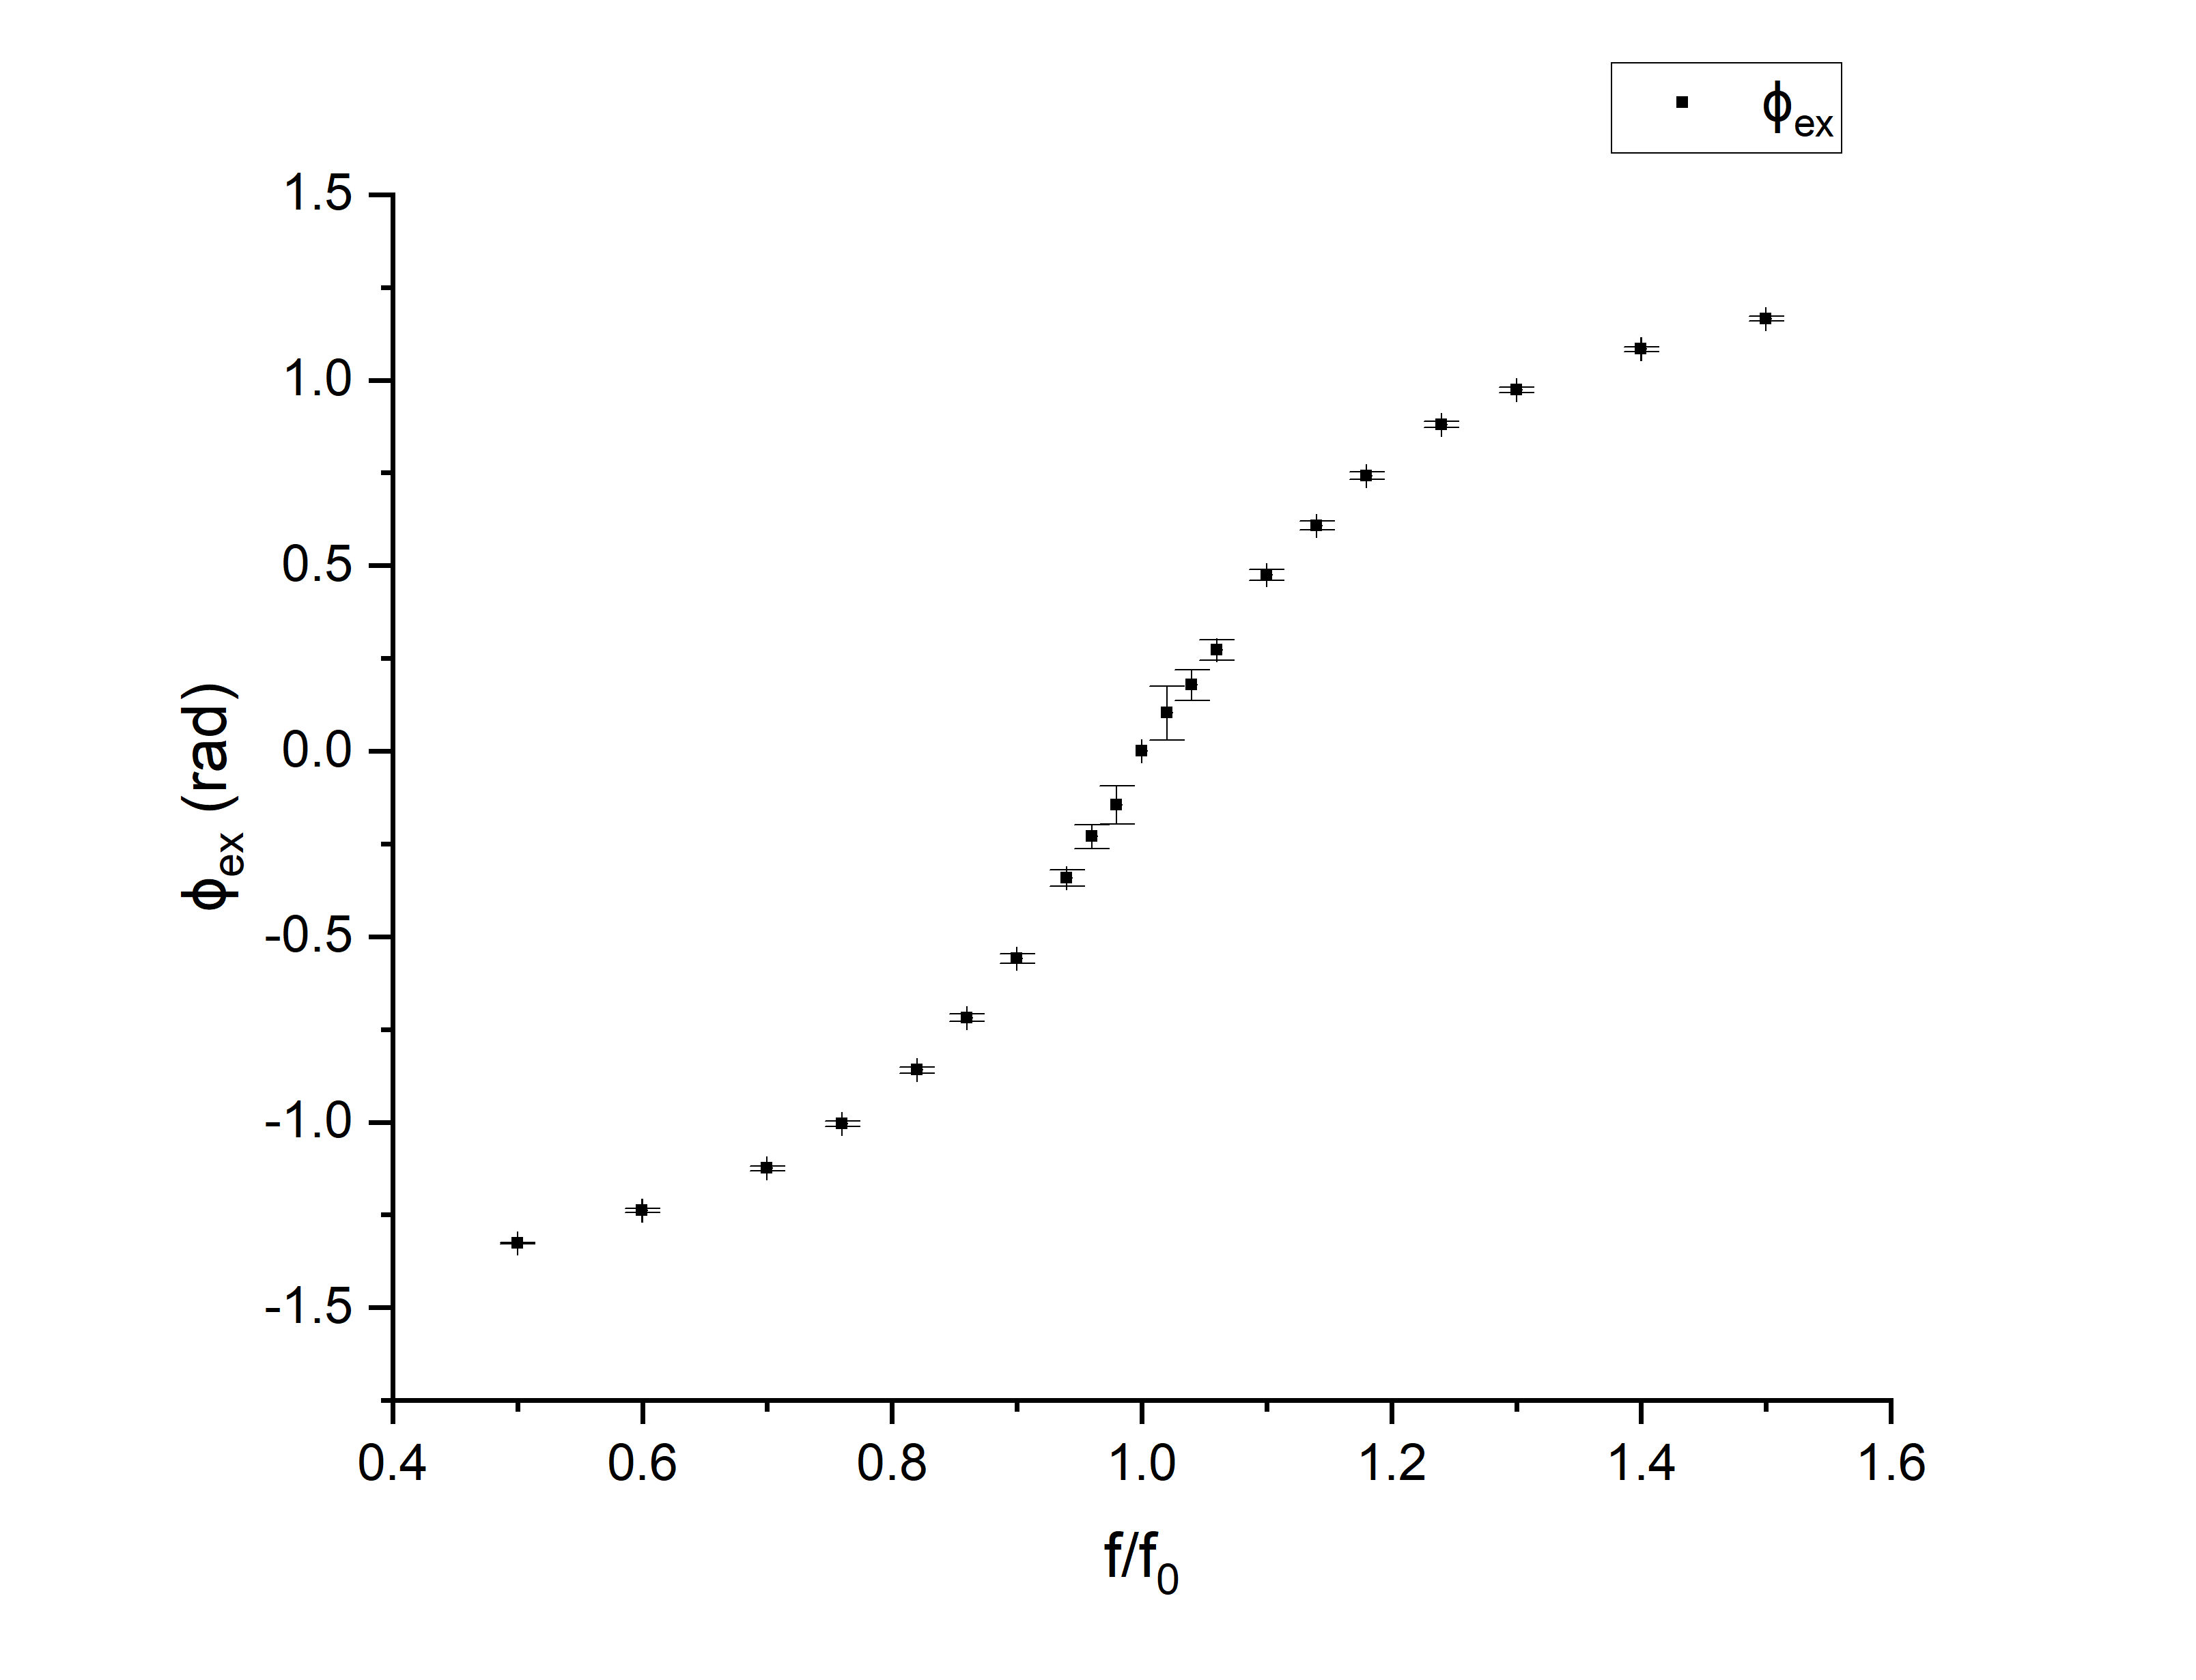
\includegraphics[scale=0.37]{phi_ex.png}
    \caption{$\varphi_\text{ex}$ vs. $f/f_0$ relation.}\label{FigPhi_ex}
\end{figure}

\subsubsection{Resonance Frequency $f_0$ and Quality Factor $Q$}

As discussed in the previous section, the experimentally estimated resonance frequency is $f_0 = 5000.000\pm 0.001\,[\text{Hz}]$. According to Eq.\eqref{eq:fres}, the theoretical resonance frequency is

$$f_{0_{theo}} = \frac{1}{2\pi\sqrt{LC}} = \frac{1}{2\pi \sqrt{0.01\times 99.82\times 10^{-9}}} = 5037.4\pm 0.2\,[\text{Hz}]$$

The relative error is thus
$$\epsilon = \frac{f_0 - f_{0_{\text{theo}}}}{f_{0_{\text{theo}}}} \times 100\% = \frac{5000.000 - 5037.4}{5037.4} \times 100\% = -0.74\,\%.$$

To find the quality factor, first find out the frequencies $f_1$, $f_2$ at which $I/I_m$ is about $1/\sqrt{2}$. Consulting Table \ref{TableResonant} and \ref{TablePhi}, we obtain that $f_1 = 4300 \text{Hz}$ and $f_2 = 5900 \text{Hz}$. Then, according to Eq.\eqref{eq:Qex}, the ``experimental'' quality factor
$$Q_{\text{ex}} = \frac{f_0}{f_2 - f_1} = \frac{5000.000}{5900.000-4300.000} = 3.125000 \pm 0.000003.$$


By Eq.\eqref{eq:Qtheo}, the ``theoretical'' quality factor
$$Q_{\text{theo}} = \frac{\sqrt{LC}}{RC} = \frac{\sqrt{0.01\times 99.82\times 10^{-9}}}{100.63\times 99.82\times 10^{-9}} = 3.1453 \pm 0.0004.$$

The relative error is thus
$$\epsilon = \frac{Q_{\text{ex}} - Q_{\text{theo}}}{Q_{\text{theo}}} \times 100\% = \frac{3.125000 - 3.1453}{3.1453} \times 100\% = 0.64\,\%.$$

\section{Conclusions and Discussion}

\subsection{$RC$, $RL$ and $RLC$ Series Circuits}

As for the \textbf{waveforms}, the waveforms recorded all assume the theoretical shape except for that in Figure \ref{FigRLL}. In Figure \ref{FigRLL}, the voltage across the capacitor does not reach the value of the supply voltage, even after it reaches the steady stage. This is probably due to the fact that the inductor is not ideal and thus at the steady stage, it will "consume" some voltage.

One drawback of the record lies in the waveform for the underdamped regime (Figure \ref{FigUnderdamp}). It seems that the period of the square wave is not large enough so as to fully display the progress of the change of the value of $U_C$.

\begin{table}[H]\centering
    \begin{tabular}{cccc}
        \toprule
                      & Experimental $\tau\,\,[\mu\text{s}]$ & Theoretical $\tau_{\text{theo}}\,\,[\mu\text{s}]$ & Relative error \\
        \midrule
        $RC$ circuit  & 12.9842 $\pm$ 0.0014                 & 10.0449 $\pm$ 0.0014                              & 29.26$\%$      \\
        $RL$ circuit  & 103.874 $\pm$ 0.014                  & 99.374 $\pm$ 0.010                                & 4.53$\%$       \\
        $RLC$ circuit & 71.43 $\pm$ 0.06                     & 31.5943 $\pm$ 0.0016                              & 126.1$\%$      \\
        \bottomrule
    \end{tabular}
    \caption{Result of time constant in $RC$, $RL$ and $RLC$ series circuits.}\label{TableResult}
\end{table}

For the measurement of the \textbf{time constant}, the results are summarized in Table \ref{TableResult}.
It can be seen that only the second item is relatively satisfying. The reason for the relatively large discrepancy of the first item can be somehow inferred from the waveform recorded (Figure \ref{FigRCC}). It can be seen that in Figure \ref{FigRCC}, the time needed for tha capacitor to get fully charged is \textbf{smaller} than that in Figure \ref{FigRLL}. This will result in \textbf{a larger relative error} in the measurement of the half-time. As to the third item, it is obvious from the huge relative error that this measurement is \textbf{wrong}. This is really strange and I look up the photos I recorded during the lab so as to find out some clues. I happened to have taken the following picture (Figure \ref{fig:error}). And based on the picture, one most probable cause I come up with is that when measuring the half-time, the scale is adjusted so that the waveform is enlarged. However, I might have \textbf{forgotten to adjust the position of the left cursor. It is not in the right position which represents the instant the source voltage is supplied, but is deflected to the left a bit}. This therefore causes the measured half-time to become much larger than its actual value and thus results in the error of the time constant measured.

\begin{figure}[H] \centering
    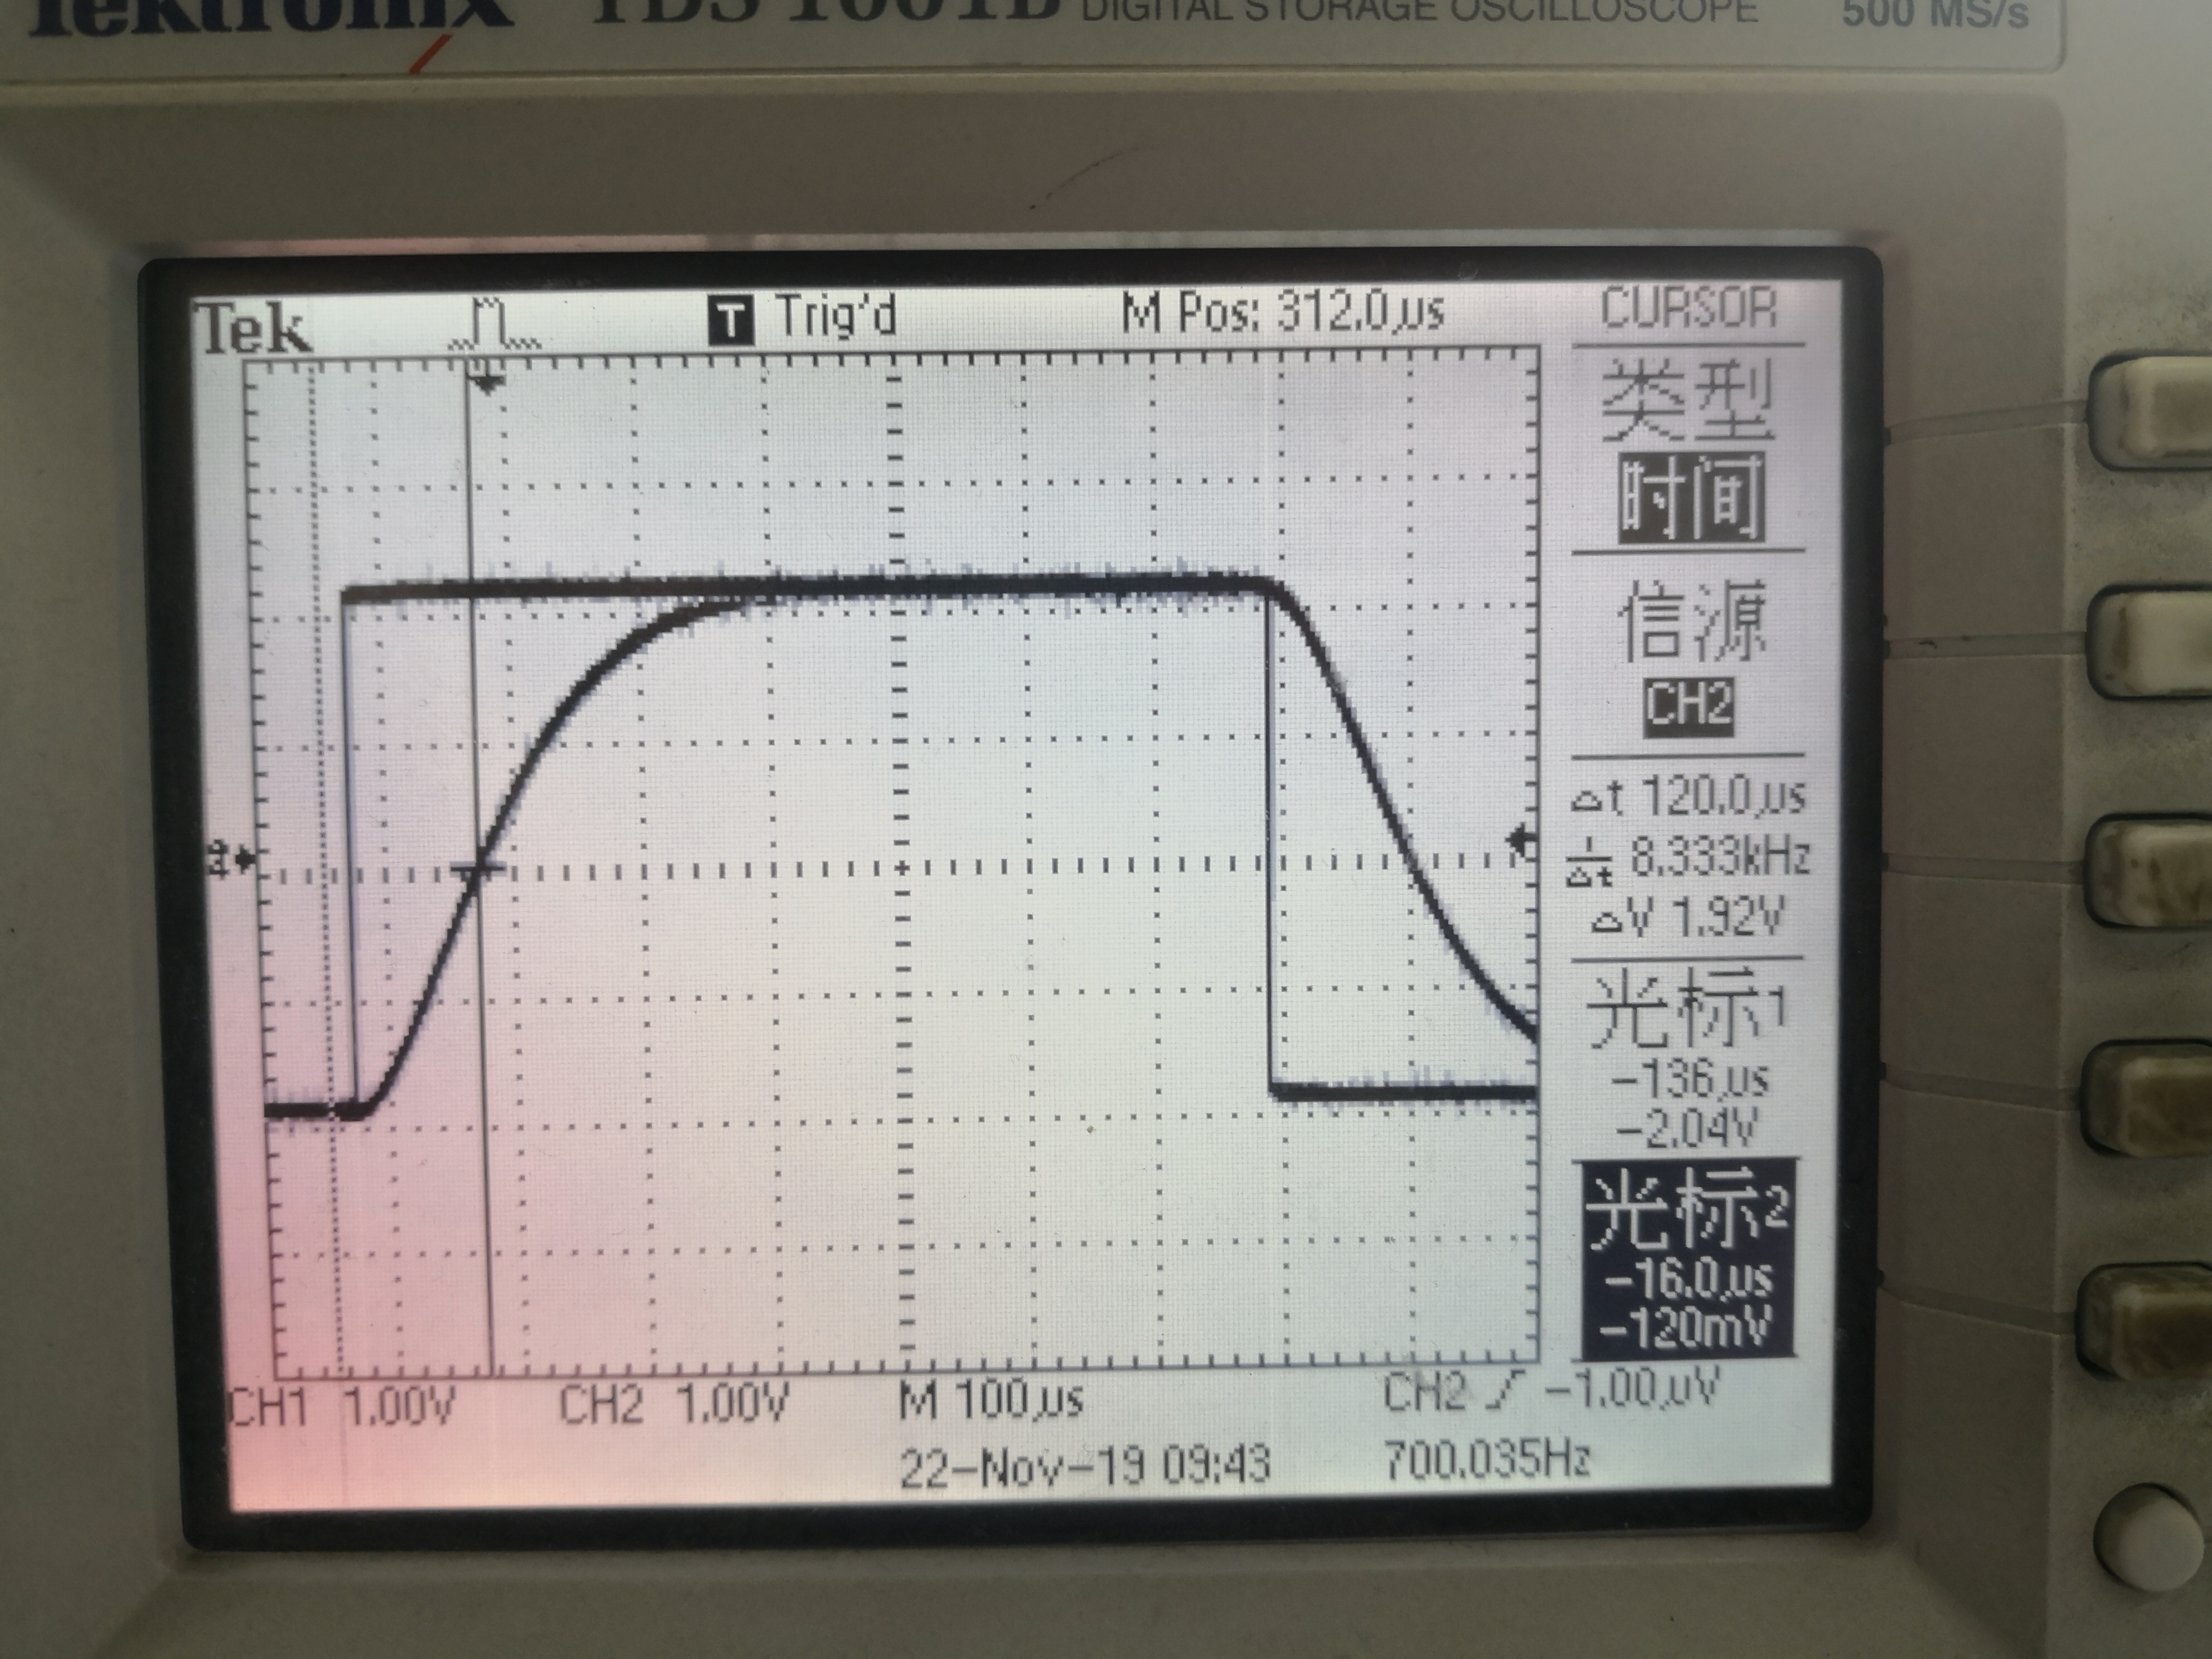
\includegraphics[width=0.45\textwidth]{6.jpg}
    \caption{One probable cause for the error.}
    \label{fig:error}
\end{figure}

\subsection{$RLC$ Resonant Circuit}


In the second part of the experiment, we studied the $RLC$ resonance circuit. The resonance curves obtained from the experiment, i.e. the $I/I_\text{m}$ vs. $f/f_0$ relation and $\varphi_\text{ex}$ vs. $f/f_0$ relation agree with the theoretical fact. The measured $\varphi_\text{ex}$ vs. $f/f_0$ relation is also in accord with the $\varphi_\text{theo}$ vs. $f/f_0$ calculated. Besides, the resonance frequency and the quality factor are found from the resonance curves. The results are summarized in Table Table \ref{tab:fQ}.

\begin{table}[H] \centering
    \begin{tabular}{cccc}
        \toprule
                           & Experimental           & Theoretical        & Relative error \% \\
        \midrule
        $f_0\,[\text{Hz}]$ & $5000.000\pm 0.001$    & $5037.4\pm 0.2$    & -0.74             \\
        $Q$                & $3.125000\pm 0.000003$ & $3.1453\pm 0.0004$ & 0.64              \\
        \bottomrule
    \end{tabular}
    \caption{Result of resonance frequency and quality factor.}
    \label{tab:fQ}
\end{table}

It can be seen that the experimental result is of relatively high accuracy. Error for the measurement of resonance frequency lies in \textbf{the choice of frequency} applied during the experiment. The \textbf{difference} between two frequencies is set to be 100 Hz. By rearrange the choice of frequency, this value can be made smaller so that a higher accuracy can be realized. Error for the measurement of quality factor originates from the fact that there is no set of data measured \textbf{exactly at the point $I/I_m = 1/\sqrt{2}$} and we can only choose the data most close to that point.

\subsection{Suggestions and Improvement}

The following suggestions may help improve the experiment:
\begin{enumerate}
    \item Do remember to \textbf{scale up the waveform} so that the $T_1/2$ point can be reached more exactly.
    \item The measured value of $U_R$ is not stable, so maybe we should \textbf{measure three times} and take the average \textbf{at some significant point} such as the value at the maximum.
    \item To find the resonance frequency more precisely, it is suggested that we can \textbf{calculate the theoretical value first} and then \textbf{set the frequencies based on the theoretical value}. In this way the choice of frequency can be made more reasonable (more data points near the theoretical value).
\end{enumerate}

\subsection{Conclusions}

To sum up, in this lab, the waveforms of the $RC$, $RL$ and $RLC$ series circuits are verified and the corresponding time constants are found out. Besides, the phenomenon of electromagnetic resonance is studied. The resonance curves are drawn based on measurement and calculations and the resonance frequency and the quality factor is estimated. Except for the time constant of the $RLC$ series circuit, other experimental results are acceptable and conform to the theoretical fact. The sources and causes for the errors, especially the error for the time constant of the $RLC$ circuit, are identified and explained. In general, the objectives of lab are fulfilled.

\begin{thebibliography}{1}

    \bibitem{manual} VP241 Exercise 5: RC, RL, and RLC Circuits, UM-SJTU Joint Institute.

\end{thebibliography}

\newpage

\appendix

\section{Measurement Uncertainty Analysis}

\subsection{Uncertainty of Data for $RC$ Circuit}
For $\tau = \frac{T_{1/2}}{\ln 2}$, the uncertainty is
$$u_\tau = \frac{\partial \tau}{\partial T_{1/2}}u_{T_{1/2}} = \frac{u_{T_{1/2}}}{\ln 2} = \frac{0.001}{\ln 2} = 0.0014\,\,[\mu\text{s}].$$

For $\tau_{\text{theo}} = RC$, the uncertainty is
\begin{align*}
    u_{\tau_{\text{theo}}} & = \sqrt{(\frac{\partial \tau_{\text{theo}}}{\partial R}u_R)^2+(\frac{\partial \tau_{\text{theo}}}{\partial C}u_C)^2} = \sqrt{(Cu_R)^2 + (Ru_C)^2} \\
                           & = \sqrt{(99.82\times0.01)^2 + (100.63\times0.01)^2} \times 10^{-3}                                                                                \\
                           & = 0.0014\,\,[\mu\text{s}].
\end{align*}

\subsection{Uncertainty of Data for $RL$ Circuit}
For $\tau = \frac{T_{1/2}}{\ln 2}$, the uncertainty is
$$u_\tau = \frac{\partial \tau}{\partial T_{1/2}}u_{T_{1/2}} = \frac{u_{T_{1/2}}}{\ln 2} = \frac{0.01}{\ln 2} = 0.014\,\,[\mu\text{s}].$$

For $\tau_{\text{theo}} = \frac{L}{R}$, the uncertainty is
\begin{align*}
    u_{\tau_{\text{theo}}} & = \sqrt{(\frac{\partial \tau_{\text{theo}}}{\partial R}u_R)^2+(\frac{\partial \tau_{\text{theo}}}{\partial L}u_L)^2} = \sqrt{(-\frac{L}{R^2}u_R)^2 + (\frac{u_L}{R})^2} \\
                           & = \sqrt{\bigg(-\frac{0.01\times0.01}{100.63^2}\bigg)^2 + \bigg(\frac{0}{100.63}\bigg)^2}                                                                                \\
                           & = 0.010\,\,[\mu\text{s}].
\end{align*}

\subsection{Uncertainty of Data for $RLC$ Circuit}
For $\tau = T_{1/2}/1.68$, the uncertainty is
$$u_\tau = \frac{\partial \tau}{\partial T_{1/2}}u_{T_{1/2}} = \frac{u_{T_{1/2}}}{1.68} = \frac{0.1}{1.68} = 0.06\,\,[\mu\text{s}].$$

For $\tau = \sqrt{LC}$, the uncertainty is
\begin{align*}
    u_{\tau_{\text{theo}}} & = \sqrt{(\frac{\partial \tau_{\text{theo}}}{\partial L}u_L)^2 + (\frac{\partial \tau_{\text{theo}}}{\partial C}u_C)^2} = \sqrt{\bigg(\frac{1}{2}\sqrt{\frac{C}{L}}u_L\bigg)^2 + \bigg(\frac{1}{2}\sqrt{\frac{L}{C}}u_C\bigg)^2} \\
                           & = \frac{1}{2}\sqrt{\frac{L}{C}}u_C = \bigg(\frac{1}{2}\sqrt{\frac{0.01}{99.82\times10^{-9}}}\times 0.01 \times 10^{-9}\bigg) \times 10^{6}                                                                                      \\
                           & = 0.0016\,\,[\mu\text{s}].
\end{align*}

\subsection{Uncertainty of Data for $RLC$ Resonant Circuit}

\subsubsection*{Uncertainty of $f/f_0$}

For $f/f_0$, the uncertainty
$$u_{f/f_0} = \sqrt{(\frac{\partial f/f_0}{\partial f}u_f)^2 + (\frac{\partial f/f_0}{\partial f_0}u_{f_0})^2} = \sqrt{(\frac{u_f}{f_0})^2 + (-\frac{f}{f_0^2}u_{f_0})^2}.$$

Take the first set of data as an example,

\begin{align*}
    u_{f/f_0} & = \sqrt{(\frac{u_f}{f_0})^2 + (-\frac{f}{f_0^2}u_{f_0})^2}                         \\
              & = \sqrt{(\frac{0.001}{5000.000})^2 + (-\frac{2500.000}{5000.000^2}\times 0.001)^2} \\
              & = 2\times 10^{-7}.
\end{align*}

The uncertainties for other sets of data are calculated in the same way and the results are shown in Table \ref{TableUnc}.

\subsubsection*{Uncertainty of $I/I_m$}
For $I/I_\text{m} = U_R/U_\text{m}$, the uncertainty

$$u_{I/I_\text{m}} = \sqrt{(\frac{\partial U_R/U_\text{m}}{\partial U_R}u_{U_R})^2 + (\frac{\partial U_R/U_\text{m}}{\partial U_\text{m}}u_{U_\text{m}})^2} = \sqrt{(\frac{u_{U_R}}{U_\text{m}})^2 + (-\frac{U_R}{U_\text{m}^2}u_{U_\text{m}})^2}.$$

Take the first set of data as an example,

\begin{align*}
    u_{I/I_\text{m}} & = \sqrt{(\frac{u_{U_R}}{U_\text{m}})^2 + (-\frac{U_R}{U_\text{m}^2}u_{U_\text{m}})^2} \\
                     & = \sqrt{(\frac{0.02}{3.80})^2 + (-\frac{0.920}{3.80^2}\times 0.02)^2}                 \\
                     & = 0.0014.
\end{align*}

The uncertainties for other sets of data are calculated in the same way and the results are shown in Table \ref{TableUnc}.

\subsubsection*{Uncertainty of $\varphi_\text{theo}$}
For $\varphi_\text{theo} = \tan^{-1}\bigg(\frac{2\pi fL-\frac{1}{2\pi fC}}{R}\bigg)$, the uncertainty

\begin{align*}
    u_{\varphi_\text{theo}} & = \sqrt{(\frac{\partial \varphi_\text{theo}}{\partial f}u_f)^2 + (\frac{\partial \varphi_\text{theo}}{\partial C}u_C)^2 + (\frac{\partial \varphi_\text{theo}}{\partial R}u_R)^2}                                                                                                                                               \\
                            & = \sqrt{\left( \frac{R\big(2\pi L +\frac{1}{2\pi f^2 C}\big)}{R^2 + \big(2\pi fL - \frac{1}{2\pi fC}\big)^2} u_f \right)^2 + \left( \frac{R}{2\pi fC^2\big[R^2+\big(2\pi fL - \frac{1}{2\pi fC}\big)^2\big]} u_C \right)^2 + \left(-\frac{2\pi fL-\frac{1}{2\pi fC}}{R^2+\big(2\pi fL-\frac{1}{2\pi fC}\big)^2} u_R \right)^2}.
\end{align*}

Take the first set of data as an example,

\begin{align*}
    u_{\varphi_\text{theo}} = & \sqrt{\left( \frac{100.63\times\big(2\pi\times0.01 +\frac{1}{2\pi\times 1000^2\times 99.82}\big)}{100.63^2 + \big(2\pi\times 1000\times 0.01 - \frac{1}{2\pi\times 1000\times 99.82}\big)^2} \right)^2 +} \\
                              & \overline{\left( \frac{100.63}{2\pi\times 1000\times 99.82^2\times\big[100.63^2+\big(2\pi\times1000\times0.01 - \frac{1}{2\pi\times1000\times99.82}\big)^2\big]} \right)^2 +}                             \\
                              & \overline{\left( \frac{2\pi\times 1000\times0.01-\frac{1}{2\pi\times 1000\times99.82}}{100.63^2+\big(2\pi\times 1000\times0.01-\frac{1}{2\pi\times 1000\times99.82}\big)^2} \right)^2}                    \\
                              & = 0.00003\,[\text{rad}].
\end{align*}

The uncertainties for other sets of data are calculated in the same way and the results are shown in Table \ref{TableUnc}.


\subsubsection*{Uncertainty of $\varphi_\text{ex}$}
For $\varphi_\text{ex}=cos^{-1}(\frac{U_R}{U_m})$, the uncertainty

$$u_{\varphi_\text{ex}} = \sqrt{(\frac{\partial \varphi_\text{ex}}{\partial U_R}u_{U_\text{R}})^2 + (\frac{\partial \varphi_\text{ex}}{\partial U_m}u_{U_\text{m}})^2} = \sqrt{(\frac{-1}{\sqrt{U_m^2-U_R^2}}u_{U_\text{R}})^2 + (\frac{U_R}{U_m\sqrt{U_m^2-U_R^2}}u_{U_\text{m}})^2}.$$

Take the first set of data as an example,

\begin{align*}
    u_{\varphi_\text{ex}} & = \sqrt{(\frac{-1}{\sqrt{U_m^2-U_R^2}}u_{U_\text{R}})^2 + (\frac{U_R}{U_m\sqrt{U_m^2-U_R^2}}u_{U_\text{m}})^2}                                   \\
                          & = \sqrt{(\frac{-1}{\sqrt{3.80^2-0.920^2}}\times 0.002)^2 + (\frac{0.920}{3.80\times\sqrt{3.80^2-0.920^2}}\times 0.02)^2} = 0.0014\,[\text{rad}].
\end{align*}


The uncertainties for other sets of data are calculated in the same way and the results are shown in Table \ref{TableUnc}.

\begin{table}[H]\centering
    \begin{tabular}{ccccc}
        \toprule
           & $u_{f/f_0}$ & $u_{I/I_\text{m}}$ & $u_{\varphi_\text{theo}}\,[\text{rad}]$ & $u_{\varphi_\text{ex}}\,[\text{rad}]$ \\
        \midrule
        1  & 0.0000002   & 0.0014             & 0.00003                                 & 0.0014                                \\
        2  & 0.0000002   & 0.006              & 0.00005                                 & 0.006                                 \\
        3  & 0.0000002   & 0.006              & 0.00008                                 & 0.006                                 \\
        4  & 0.0000003   & 0.006              & 0.00011                                 & 0.007                                 \\
        5  & 0.0000003   & 0.006              & 0.00015                                 & 0.008                                 \\
        6  & 0.0000003   & 0.007              & 0.00019                                 & 0.010                                 \\
        7  & 0.0000003   & 0.007              & 0.0002                                  & 0.013                                 \\
        8  & 0.0000003   & 0.007              & 0.0003                                  & 0.02                                  \\
        9  & 0.0000003   & 0.007              & 0.0003                                  & 0.03                                  \\
        10 & 0.0000003   & 0.007              & 0.0003                                  & 0.05                                  \\
        11 & 0.0000003   & 0.007              & 0.0003                                  & /                                     \\
        12 & 0.0000003   & 0.007              & 0.0003                                  & 0.07                                  \\
        13 & 0.0000003   & 0.007              & 0.0003                                  & 0.04                                  \\
        14 & 0.0000003   & 0.007              & 0.0003                                  & 0.03                                  \\
        15 & 0.0000003   & 0.007              & 0.0002                                  & 0.015                                 \\
        16 & 0.0000003   & 0.007              & 0.00018                                 & 0.012                                 \\
        17 & 0.0000003   & 0.007              & 0.00014                                 & 0.010                                 \\
        18 & 0.0000003   & 0.006              & 0.00011                                 & 0.008                                 \\
        19 & 0.0000003   & 0.006              & 0.00008                                 & 0.007                                 \\
        20 & 0.0000003   & 0.006              & 0.00006                                 & 0.007                                 \\
        21 & 0.0000004   & 0.006              & 0.00004                                 & 0.006                                 \\
        \bottomrule
    \end{tabular}
    \caption{Uncertainty for $\varphi$, $f/f_0$ and $I/I_\text{m}$.}\label{TableUnc}
\end{table}

\subsubsection*{Uncertainty of $f_{0_{\text{theo}}}$}

For $f_{0_\text{{theo}}} = \frac{1}{2\pi\sqrt{LC}}$, the uncertainty

\begin{align*}
    U_{f_{0_{\text{theo}}}} & = \sqrt{(\frac{\partial f_{0_{\text{theo}}}}{\partial L}u_L)^2 + (\frac{\partial f_{0_{\text{theo}}}}{\partial C}u_C)^2}                                                                     \\
                            & = \sqrt{\left[\frac{1}{2 \pi \sqrt{C}}\left(-\frac{1}{2} L^{-\frac{3}{2}}\right) u_{L}\right]^{2}+\left[\frac{1}{2 \pi \sqrt{L}}\left(-\frac{1}{2} C^{-\frac{3}{2}}\right) u_{C}\right]^{2}} \\
                            & = \sqrt{0+\left[\frac{1}{2 \pi \times \sqrt{0.01}} \times\left(-\frac{1}{2}\right) \times\left(99.82 \times 10^{-9}\right)^{-\frac{3}{2}} \times\left(0.01 \times 10^{-9}\right)\right]^{2}} \\
                            & = 0.2 \,[\text{Hz}]
\end{align*}

\subsubsection*{Uncertainty of $Q_\text{ex}$}

For $Q_\text{ex} = \frac{f_0}{f_2 - f_1}$, the uncertainty

\begin{align*}
    u_{Q_\text{ex}} & = \sqrt{(\frac{\partial Q_\text{ex}}{\partial f_0}u_{f_0})^2 + (\frac{\partial Q_\text{ex}}{\partial f_1}u_{f_1})^2 + (\frac{\partial Q_\text{ex}}{\partial f_2}u_{f_2})^2}                 \\
                    & = \sqrt{\bigg(\frac{u_{f_0}}{f_2-f_1}\bigg)^2 + \bigg(\frac{f_0}{(f_2-f_1)^2}u_{f_1}\bigg)^2 + \bigg(-\frac{f_0}{(f_2-f_1)^2}u_{f_2}\bigg)^2}                                               \\
                    & = \sqrt{\bigg(\frac{0.001}{5900.000-4300.000}\bigg)^2 + \bigg(\frac{5000.000}{(5900.000-4300.000)^2}\times0.001\bigg)^2 + \bigg(-\frac{5000.000}{(5900.000-4300.000)^2}\times0.001\bigg)^2} \\
                    & = 3 \times 10^{-6}.
\end{align*}


\subsubsection*{Uncertainty of $Q_\text{theo}$}

For $Q_\text{theo} = \frac{\sqrt{LC}}{RC}$, the uncertainty

\begin{align*}
    u_{Q_{\text{theo}}} & = \sqrt{(\frac{\partial Q_{\text{theo}}}{\partial R}u_R)^2 + (\frac{\partial Q_{\text{theo}}}{\partial C}u_C)^2} = \sqrt{(-\frac{\sqrt{LC}}{R^2C}u_R)^2 + (-\frac{\sqrt{L}}{2RC^{3/2}} u_C)^2}                                     \\
                        & = \sqrt{\bigg(-\frac{\sqrt{0.01\times 99.82\times 10^{-9}}}{100.63^2\times 99.82\times 10^{-9}}\times 0.01\bigg)^2 + \bigg(-\frac{\sqrt{0.01}}{2\times 100.63\times(99.82\times 10^{-9})^{3/2}}\times 0.01 \times 10^{-9}\bigg)^2} \\
                        & = 0.0004.
\end{align*}

\section{Data Sheet}

Please find the original data sheet attached at the end of the report.

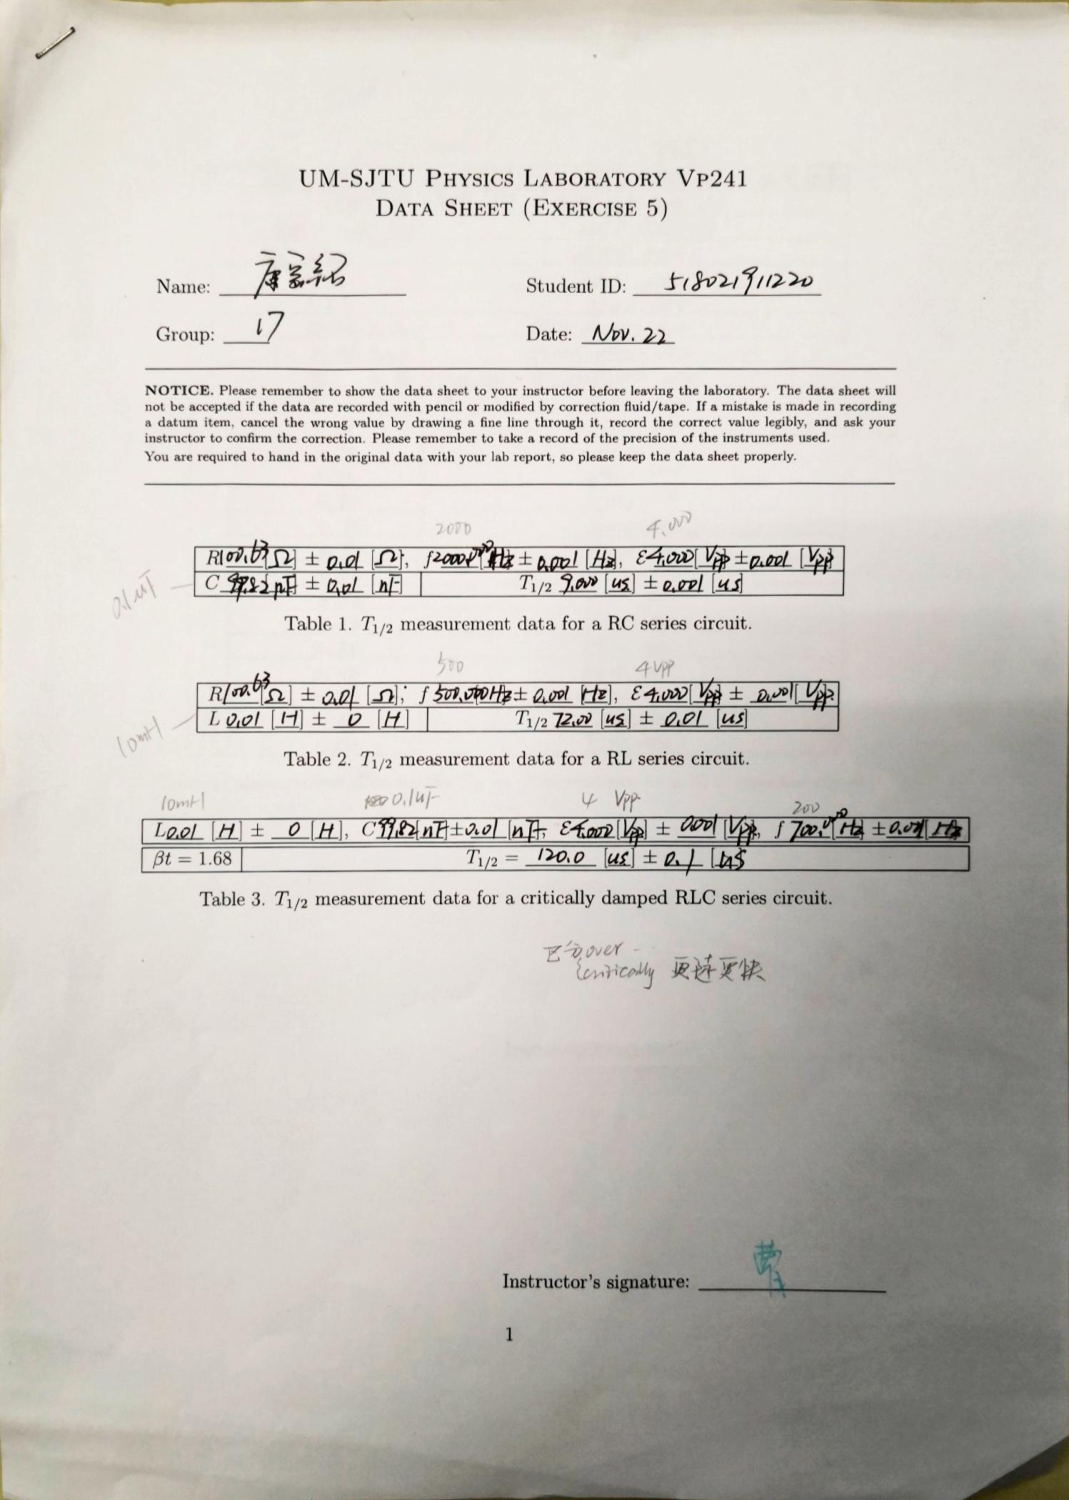
\includepdf[pages=-]{lab5datasheet.pdf}

\end{document}
